% report.tex
% main file for the project report.

\documentclass[a4paper,titlepage,11pt]{scrreprt}

% utf-8
\usepackage{polyglossia}
\setdefaultlanguage[babelshorthands]{ngerman}
\usepackage{fontspec}
\usepackage{pdfpages}

%Needed to wrap text around images, used for personas
\usepackage{wrapfig}

%Used to avoid page breaks with each chapter
\usepackage{etoolbox}
\makeatletter
\patchcmd{\chapter}{\if@openright\cleardoublepage\else\clearpage\fi}{}{}{}
\makeatother

% german names
\usepackage{ngerman}

% colored links
\usepackage{color}
\usepackage[colorlinks]{hyperref}
\definecolor{grey}{rgb}{0.2,0.2,0.2}
\definecolor{orange}{rgb}{1,0.3,0}
\definecolor{turqoise}{rgb}{0,0.7,0.5}

% code listings
\usepackage{listings}
\lstset{%
	basicstyle={\ttfamily \small},
	breaklines=true,
	commentstyle=\color{grey},
	keywordstyle=\color{orange},
	language=C,
	numbers=left,
	showspaces=false,
	stringstyle=\color{turqoise},
	xleftmargin=20pt
}

% graphics
\usepackage{graphicx}
\graphicspath{{images/}}

% fancy headers and footers
\usepackage{fancyhdr}
\pagestyle{fancy}
% clear style
\fancyhead{}
\fancyfoot{}
% new style
\renewcommand{\chaptermark}[1]{%
	\markboth{\thechapter.\ #1}{}
}
\renewcommand{\sectionmark}[1]{%
	\markright{\thesection.\ #1}{}
}
\renewcommand{\headrulewidth}{0.5pt}
\renewcommand{\footrulewidth}{0.5pt}
\fancyhead[LE,RO]{\rightmark}
\fancyhead[LO,RE]{\leftmark}
\fancyfoot[LE,RO]{\thepage}
\fancyfoot[LO,RE]{Verteilte Systeme 2 ---  Labor \\ Tobias Kerst, Patrick König und Anna-Lena Schwarzkopf}
\fancypagestyle{plain}{%
	\fancyhf{}
	\renewcommand{\headrulewidth}{0pt}
	\renewcommand{\footrulewidth}{0.5pt}
	\fancyfoot[LE,RO]{\thepage}
	\fancyfoot[LO,RE]{Verteilte Systeme 2 ---  Labor \\ Tobias Kerst, Patrick König und Anna-Lena Schwarzkopf}
}

% no indented paragraphs
\usepackage{parskip}

% sets the font for the heading to be the normal font but bold
\setkomafont{disposition}{\normalfont\bfseries}

% for verbatiminput
\usepackage{verbatim}

% not yet used
%\input{src/cmd}

\begin{document}

\thispagestyle{empty}

\titlehead{
	
\includegraphics[width=0.9\linewidth]{hska_logo}
}

\title{Verteilte Systeme 2 --- Labor}
\subtitle{Stuttr}
\author{
	Tobias Kerst (47646) \\
	Patrick König (46910)\\
	Anna-Lena Schwarzkopf (47161)
}
\date{Sommersemester 2016}
\publishers{
    \textbf{Dozent:} Prof. Dr. rer. nat. Christian Zirpins
}
\maketitle

\clearpage

\begingroup
\hypersetup{linkcolor=black}
\tableofcontents
\endgroup

\clearpage

\chapter{Konzeption und Gestaltung}

  \section{Anforderungen der Web Anwendung (Use Case Diagramm)}
    \begin{center}
      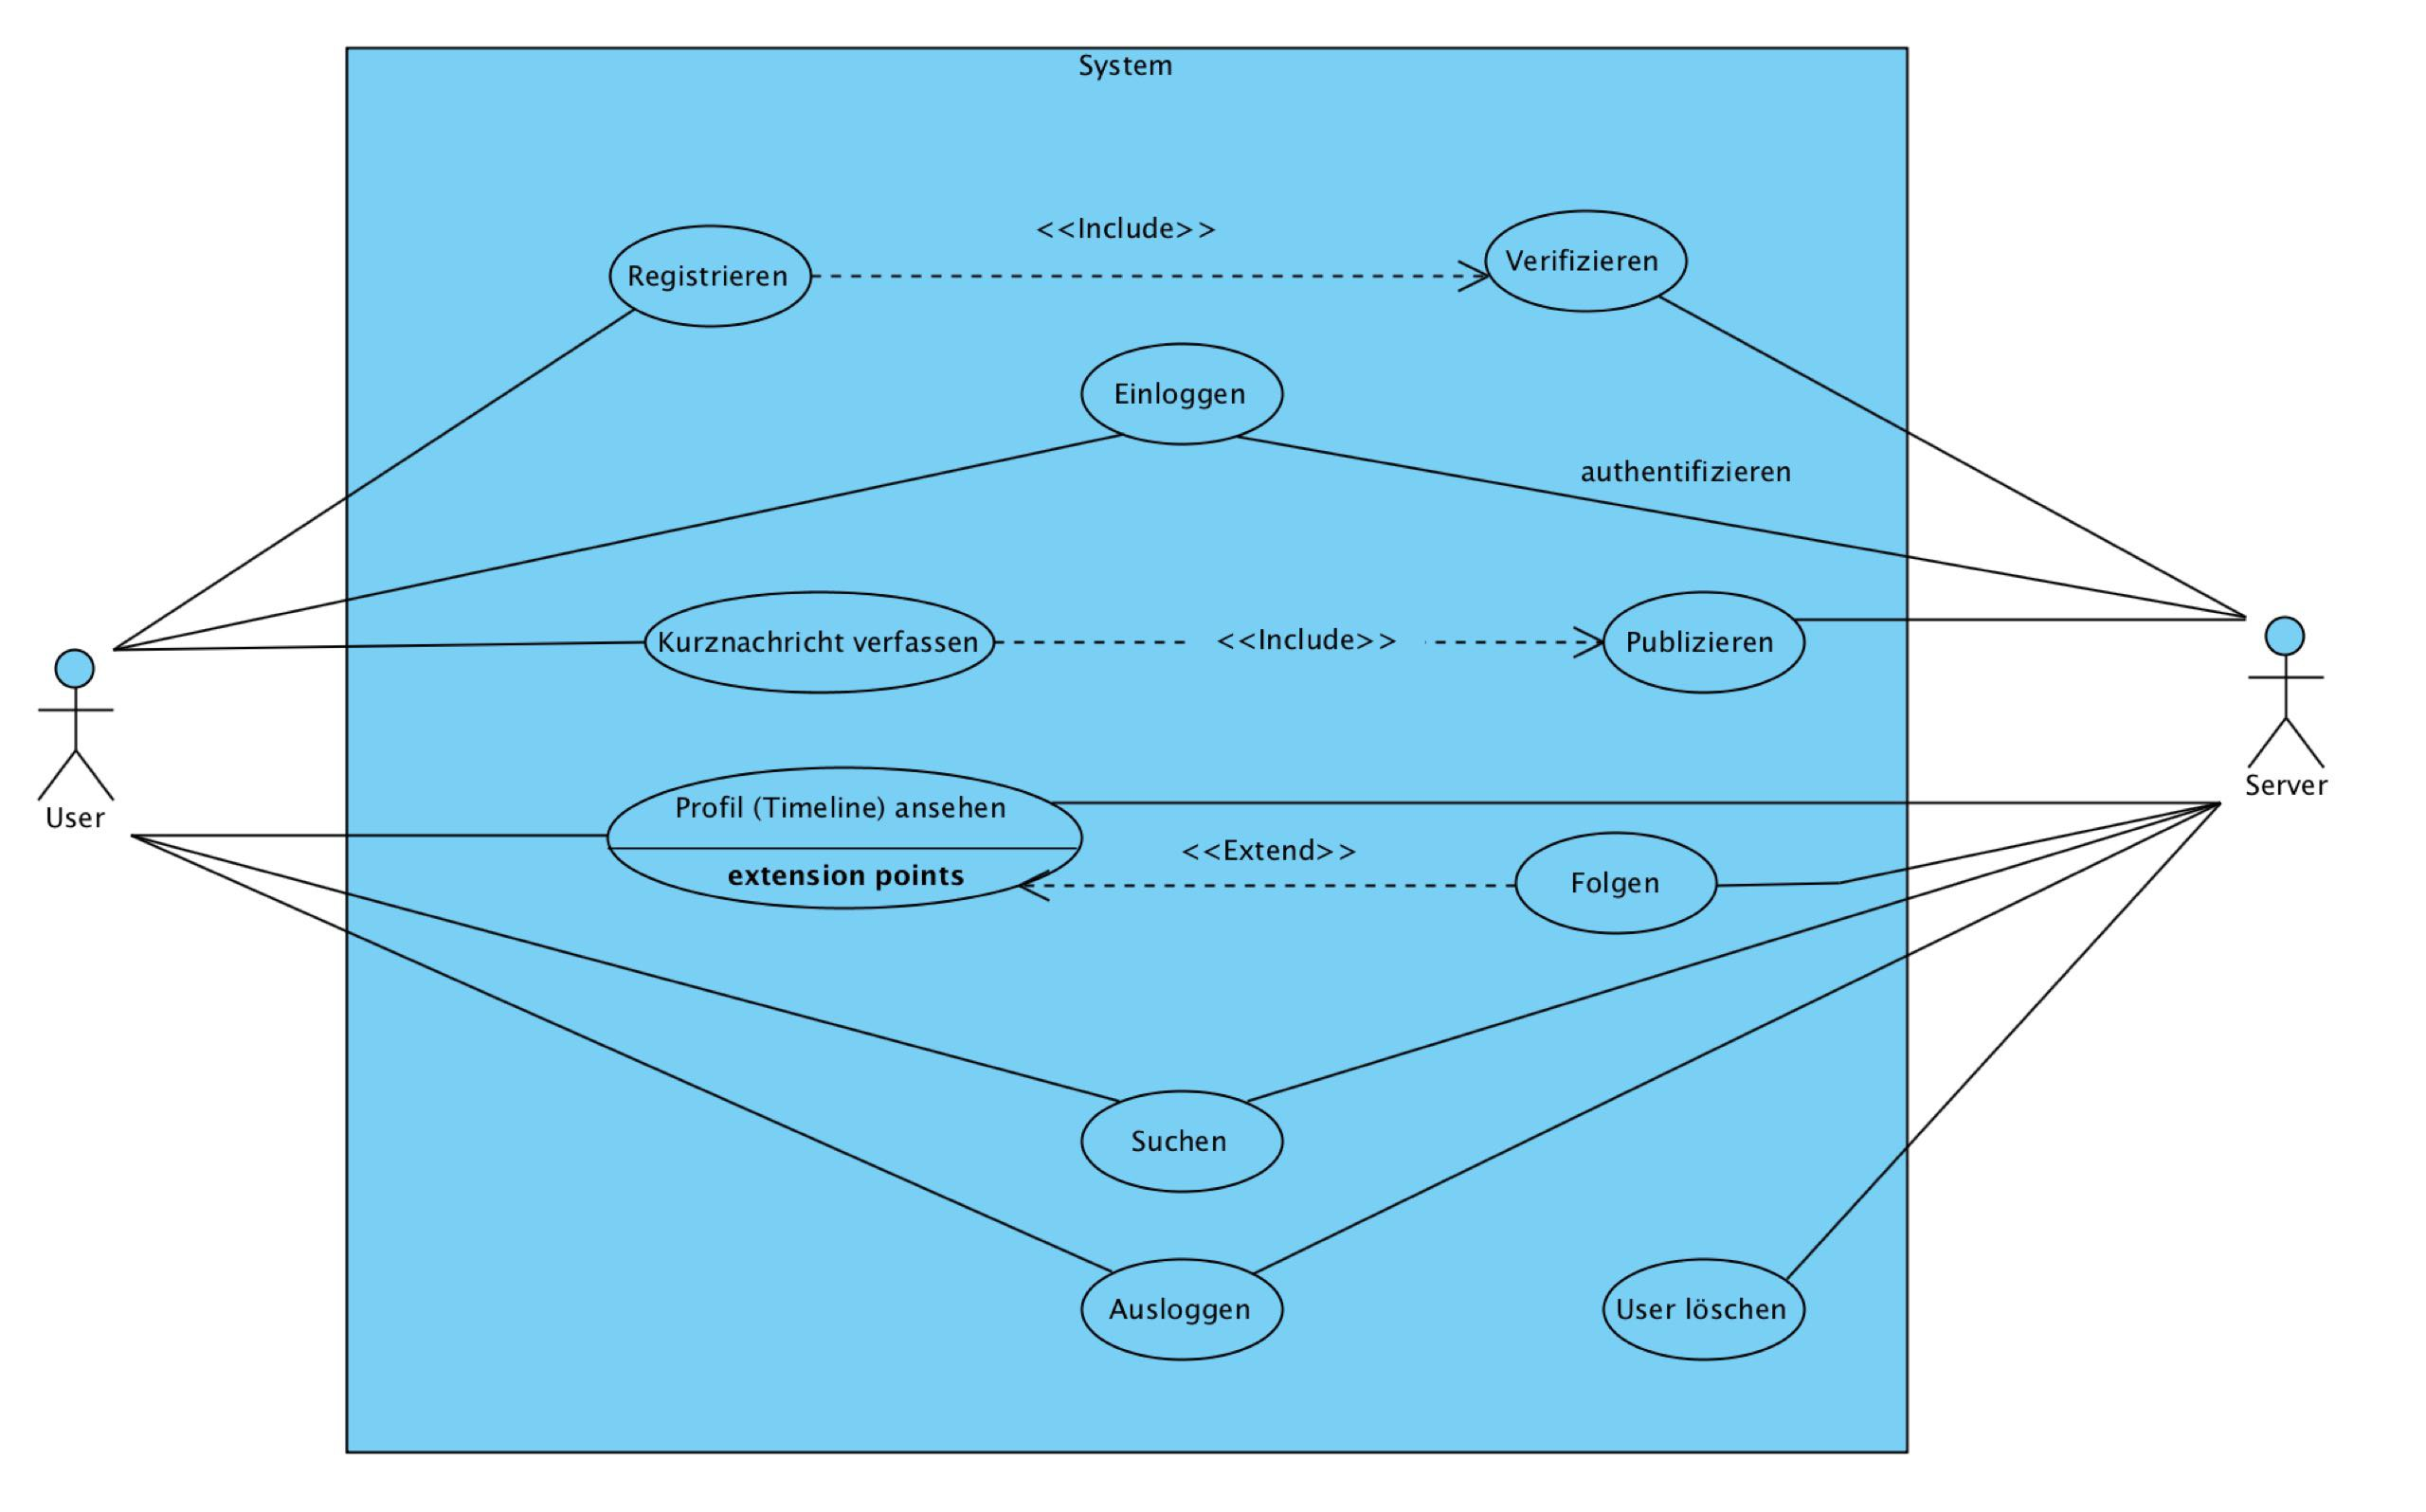
\includegraphics[width=1.0\linewidth]{usecase.jpg}
    \end{center}

\newpage
  \section{Entwurf der Seitennavigation (Zustandsdiagramm)}
    \begin{center}
      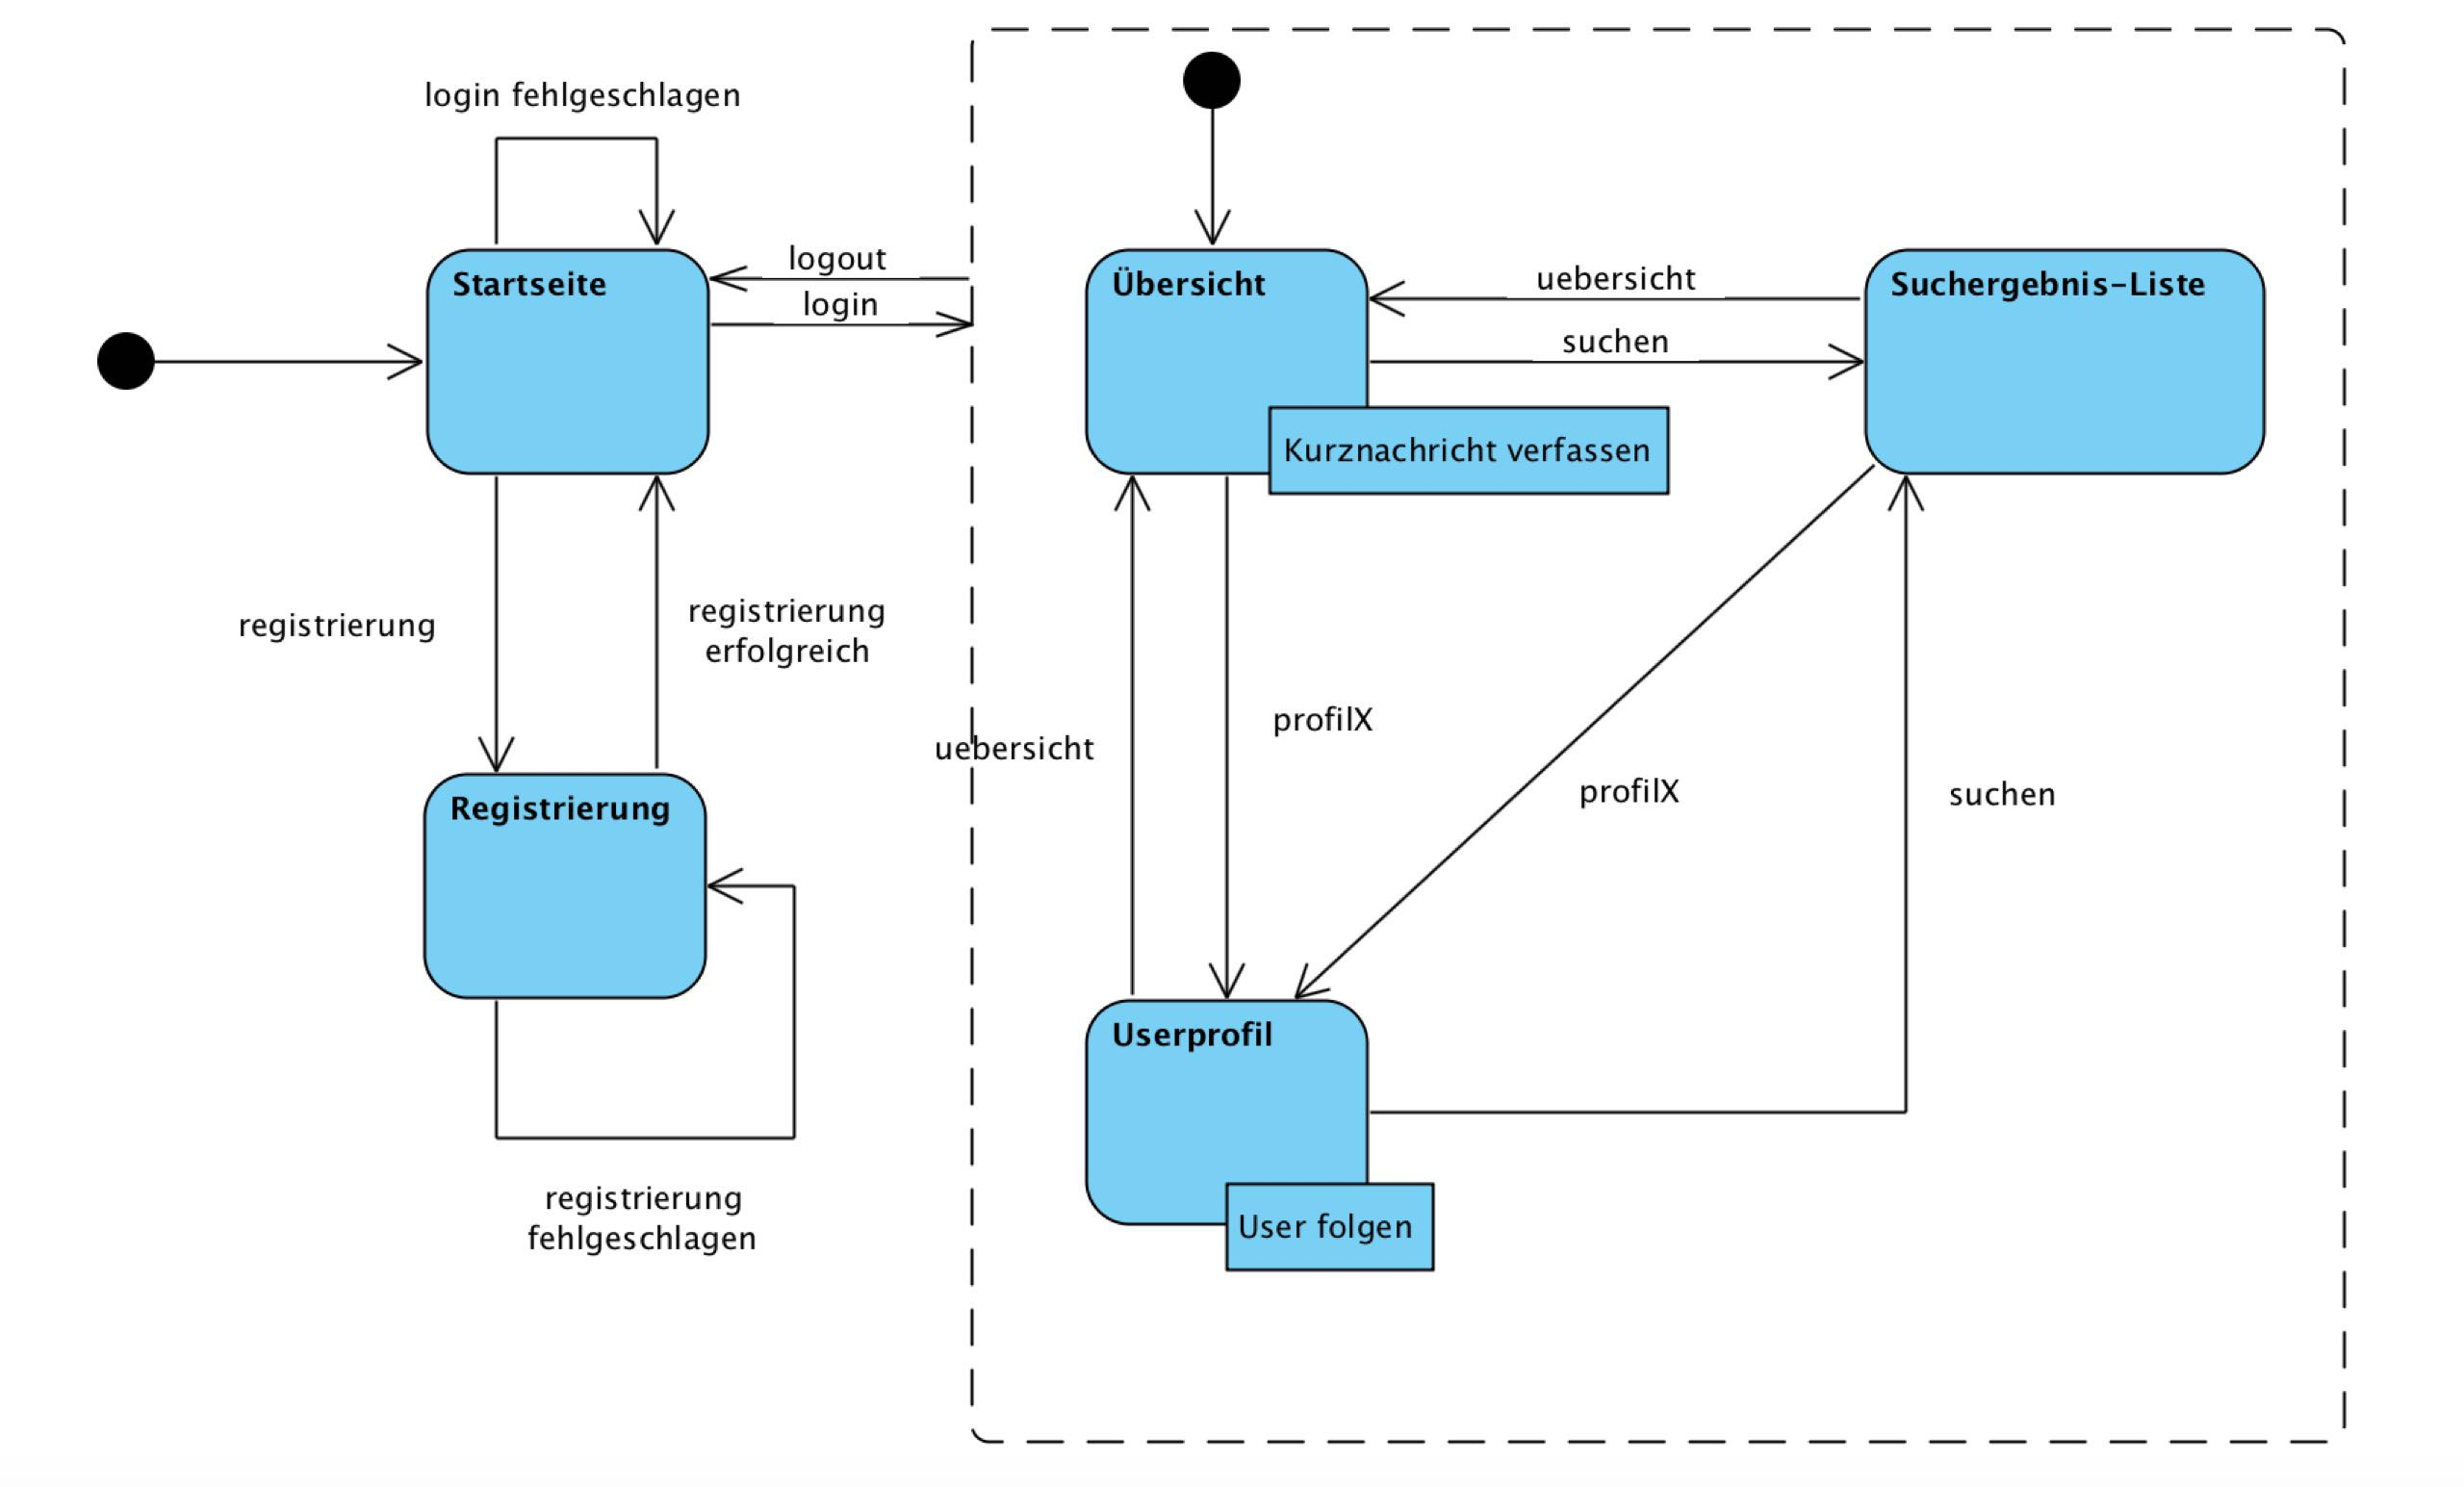
\includegraphics[width=1.0\linewidth]{zustandsdiagramm.jpg}
    \end{center}

\newpage
  \section{Mockups von Stuttr}
    \begin{center}
      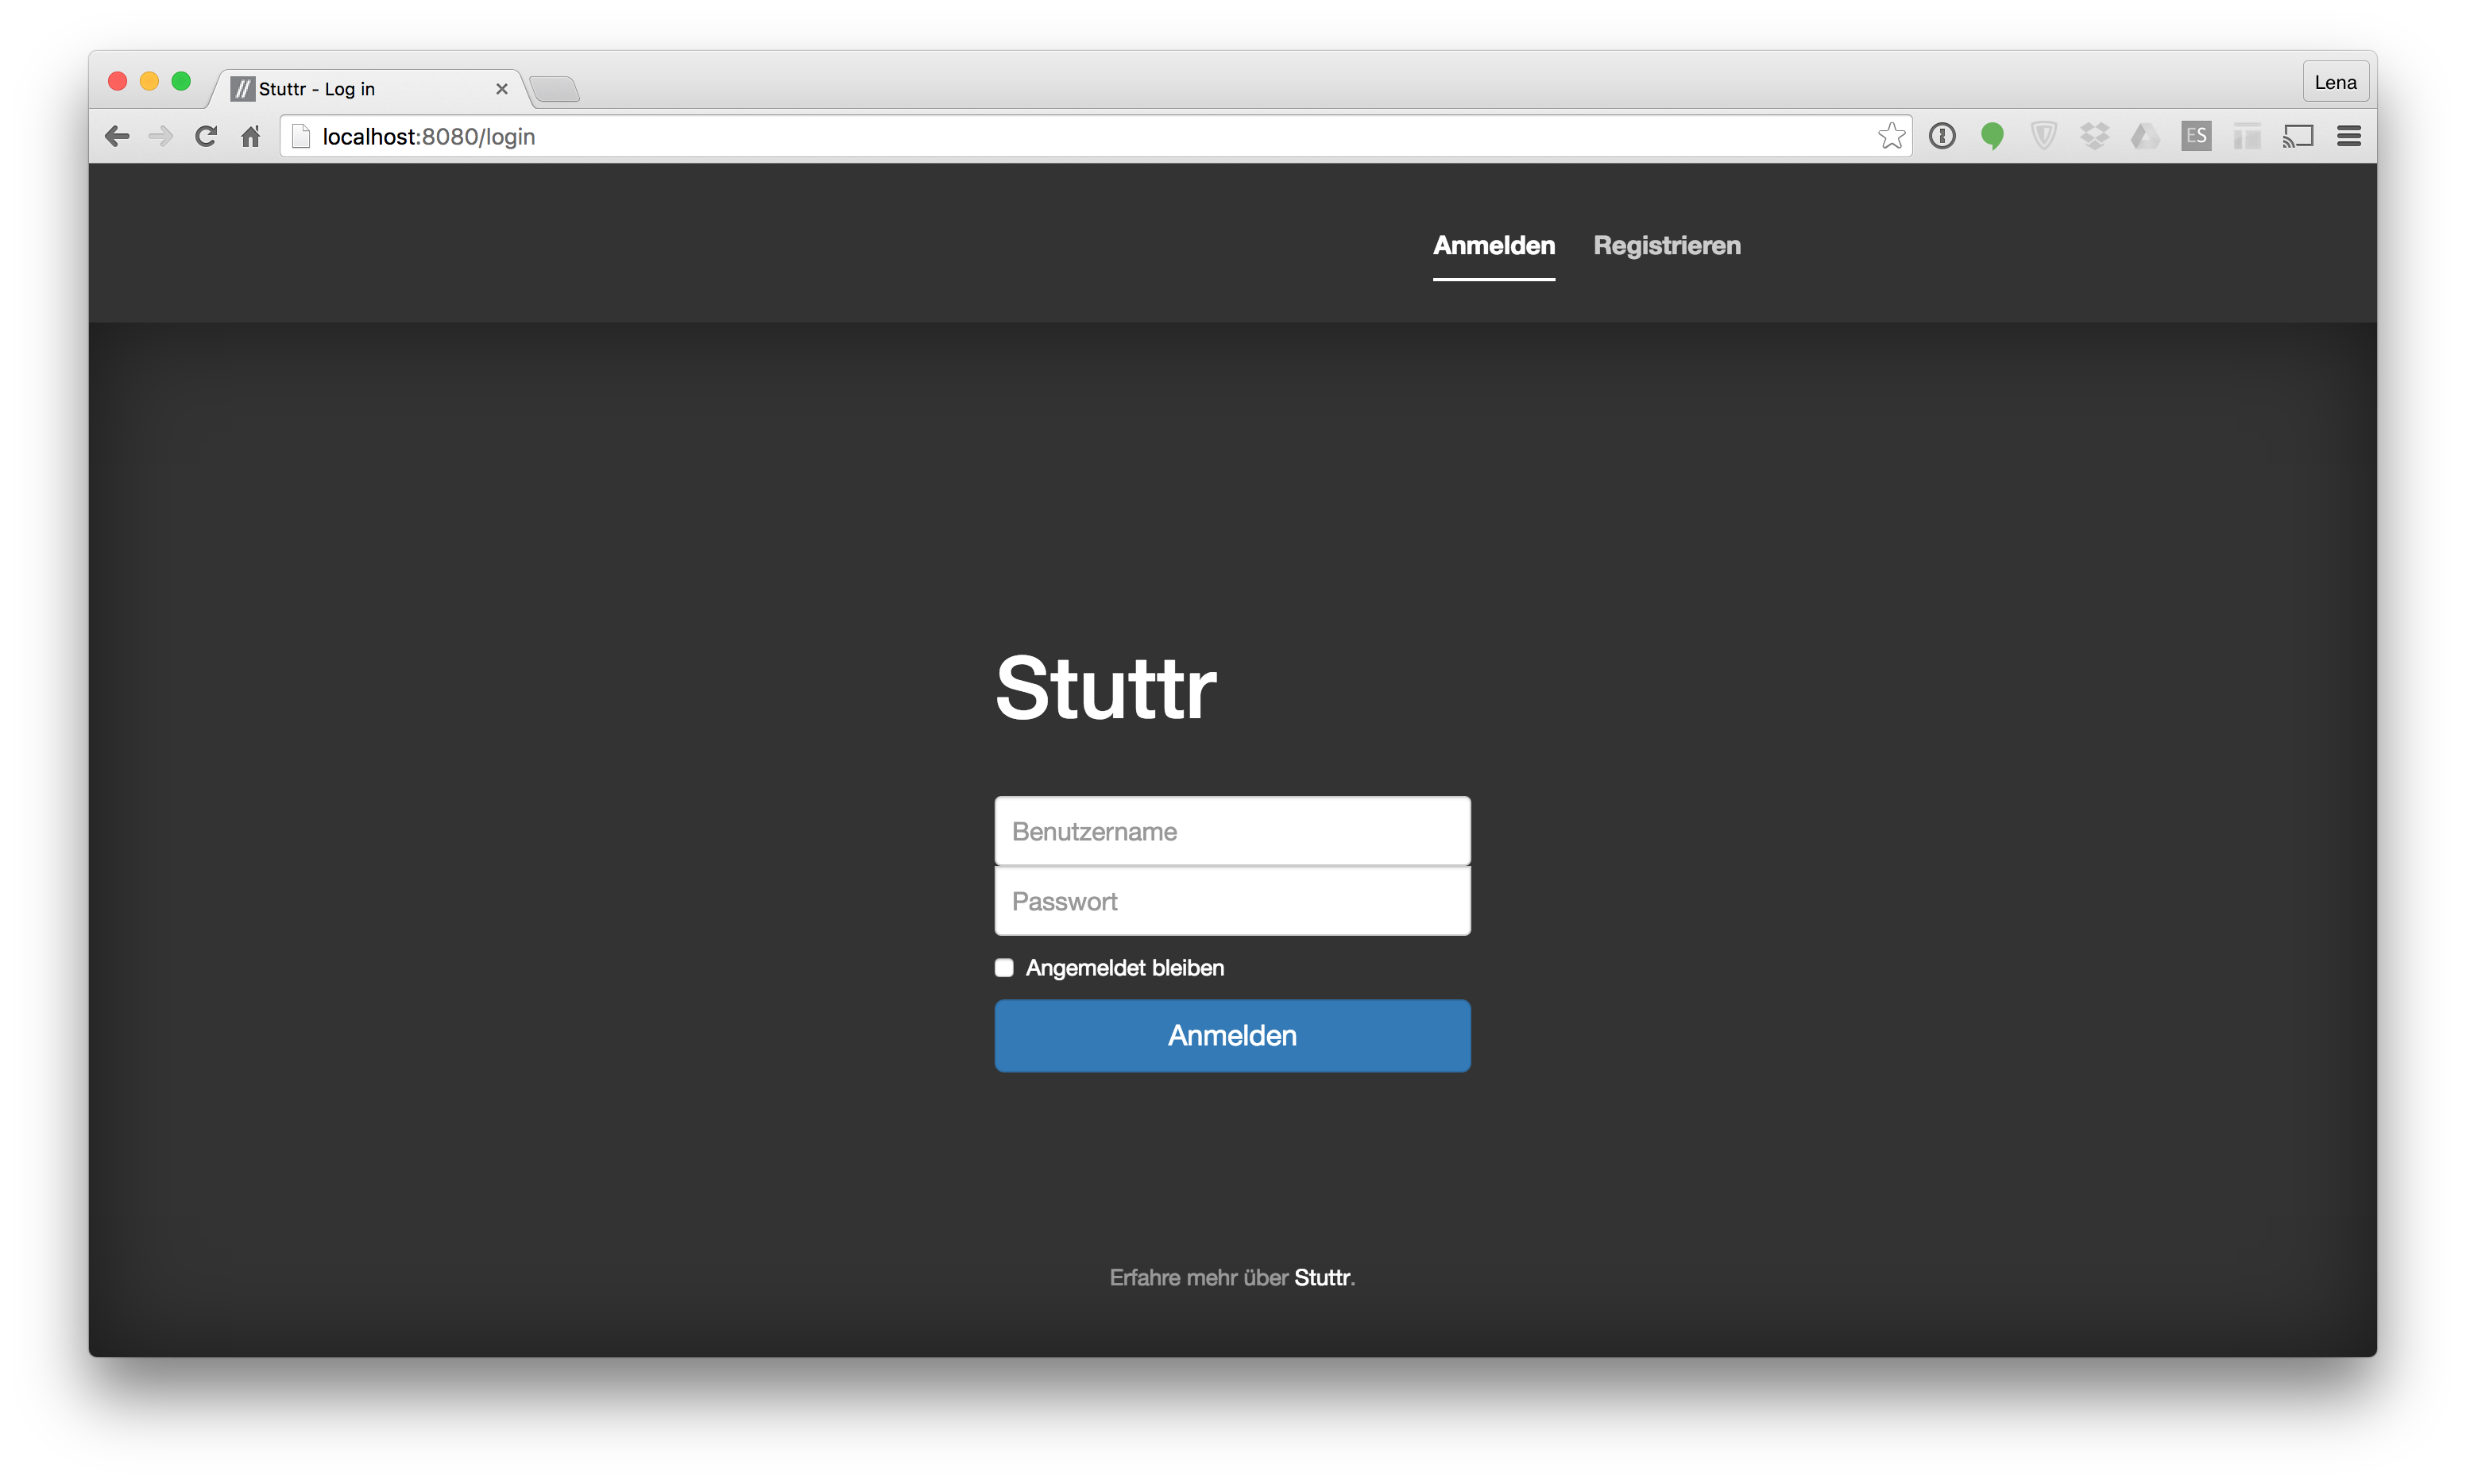
\includegraphics[width=0.75\linewidth]{login.jpg}
    \end{center}

    Der erste Screen, den der User beim Ansteuern der Seite sieht, ist der Anmelden-Screen. \\
    Hier kann der User seine Login-Daten eingeben und sich damit anmelden. \\
    In der oberen Leiste kann der User zum Punkt „Registrieren“ navigieren, sollte er noch kein Konto haben. \\
    Anhand dieses einfachen Aufbaus erkennt man auch sehr schnell, dass nur registrierte Nutzer Posts anderer Nutzer sehen können.

    \begin{center}
      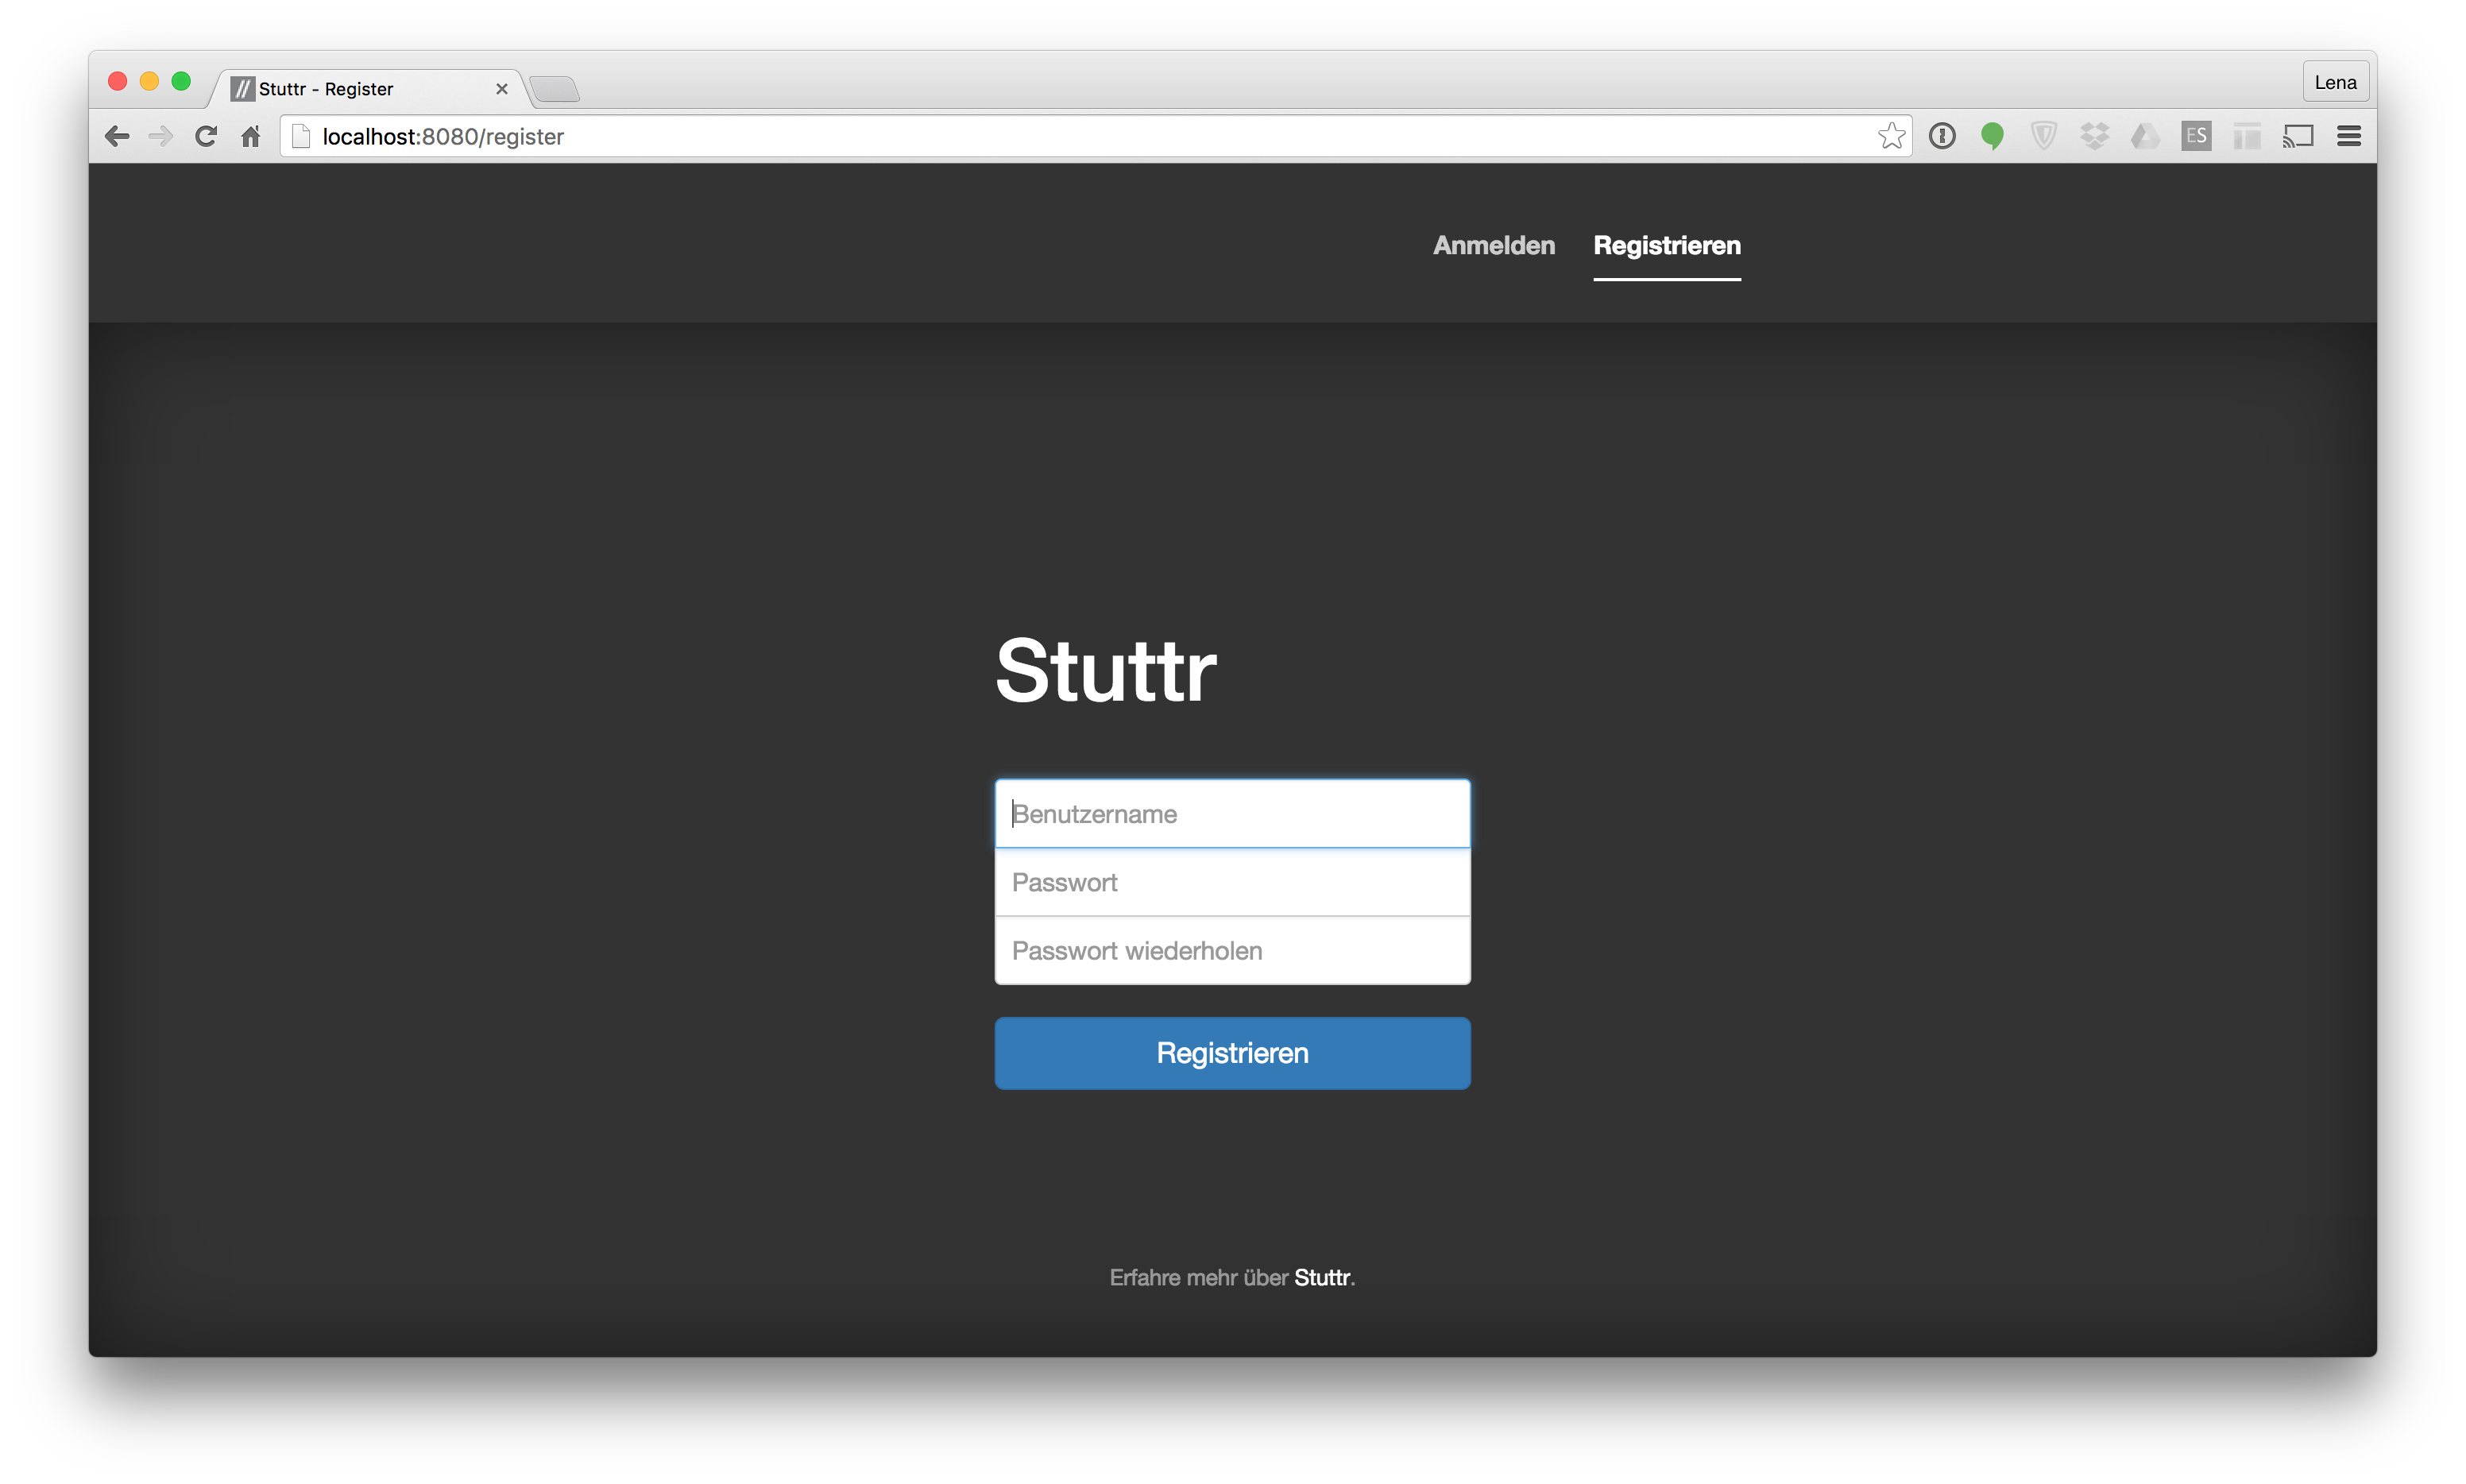
\includegraphics[width=0.75\linewidth]{register.jpg}
    \end{center}

    Der Registrieren Screen ist so einfach wie möglich gehalten und ähnelt dem „Anmelden“ Screen absichtlich, damit dem User ein bekanntes Interface die Eingabe der Daten erleichtert. \\
    Verlangt werden lediglich Username, Passwort und zur Absicherung die Wiederholung des Passwortes.

\newpage
    \begin{center}
      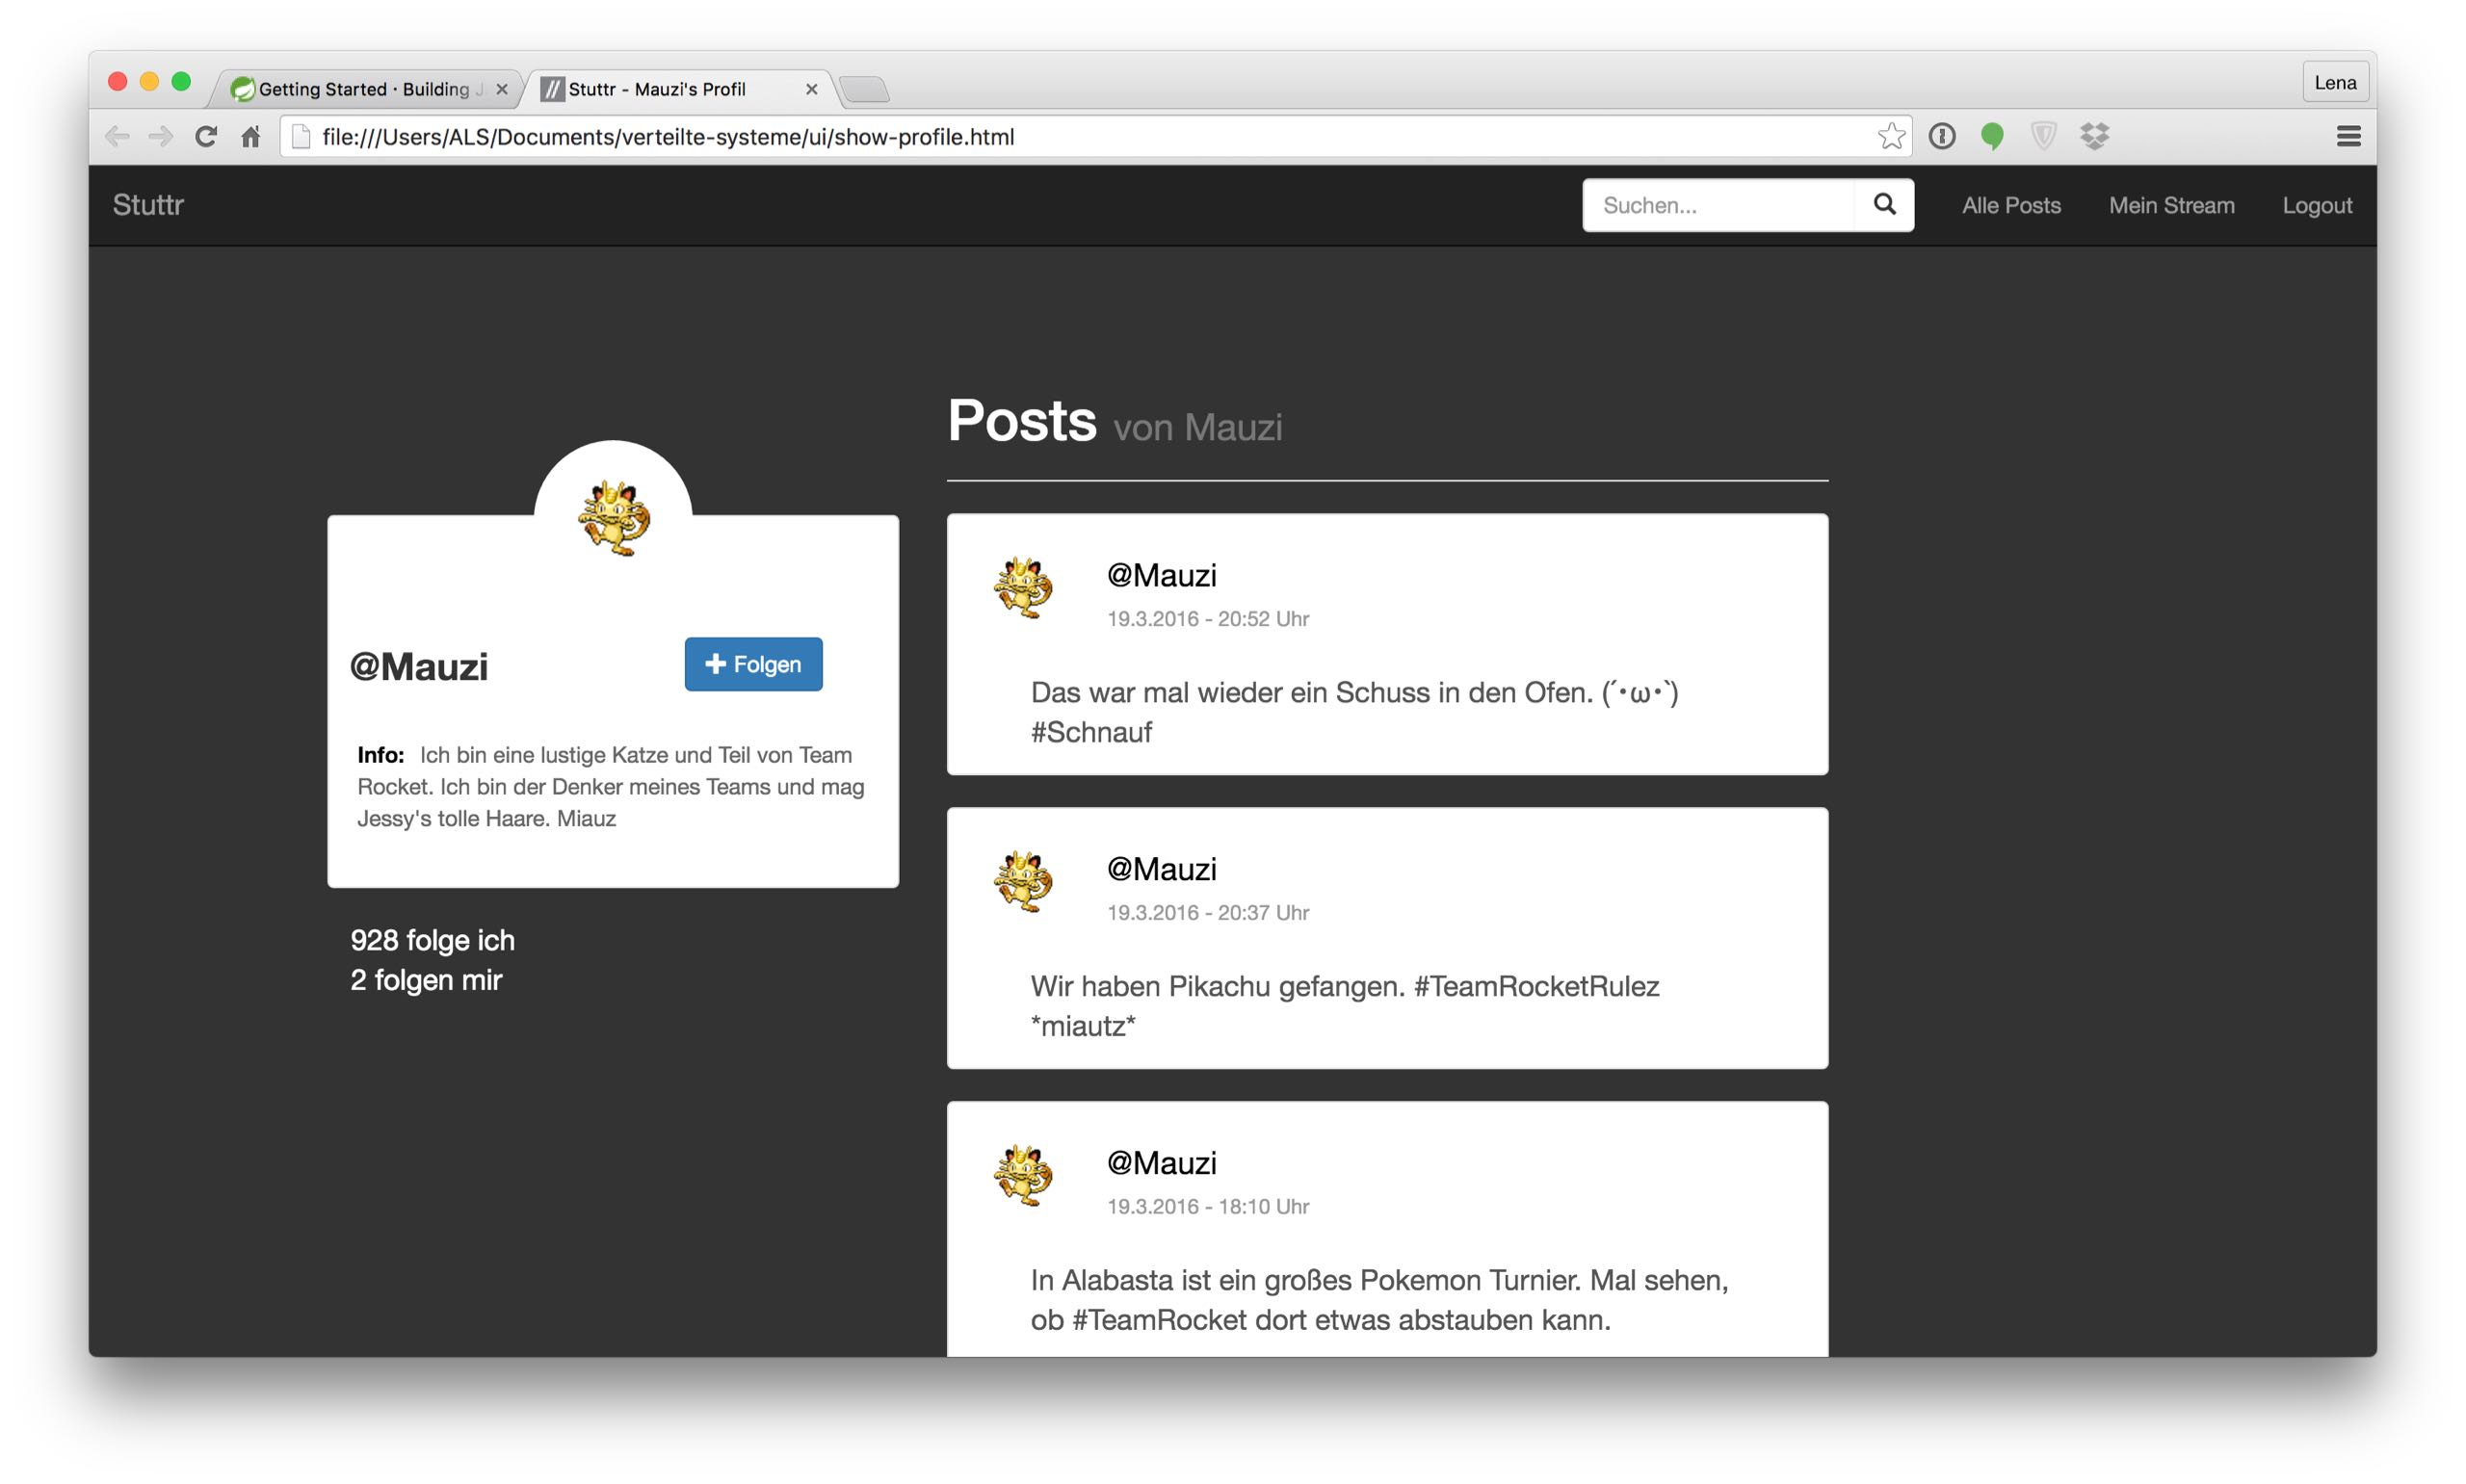
\includegraphics[width=1.0\linewidth]{show-profile.jpg}
    \end{center}

    Die Profilansicht ist sehr einfach gehalten. In der linken Spalte sind Informationen über den User enthalten, in der rechten Spalte alle Posts (in chronologischer Reihenfolge).

    Die Informationen des Users sind Folgende:
    \begin{itemize}
      \item Username
      \item Userinformationen
      \item Anzahl an Followern
      \item Anzahl an Personen, denen der User folgt
    \end{itemize}

    Zusätzlich kann man über den Button „Folgen“ dem User folgen, also dessen Posts abonnieren.

\newpage
    \begin{center}
      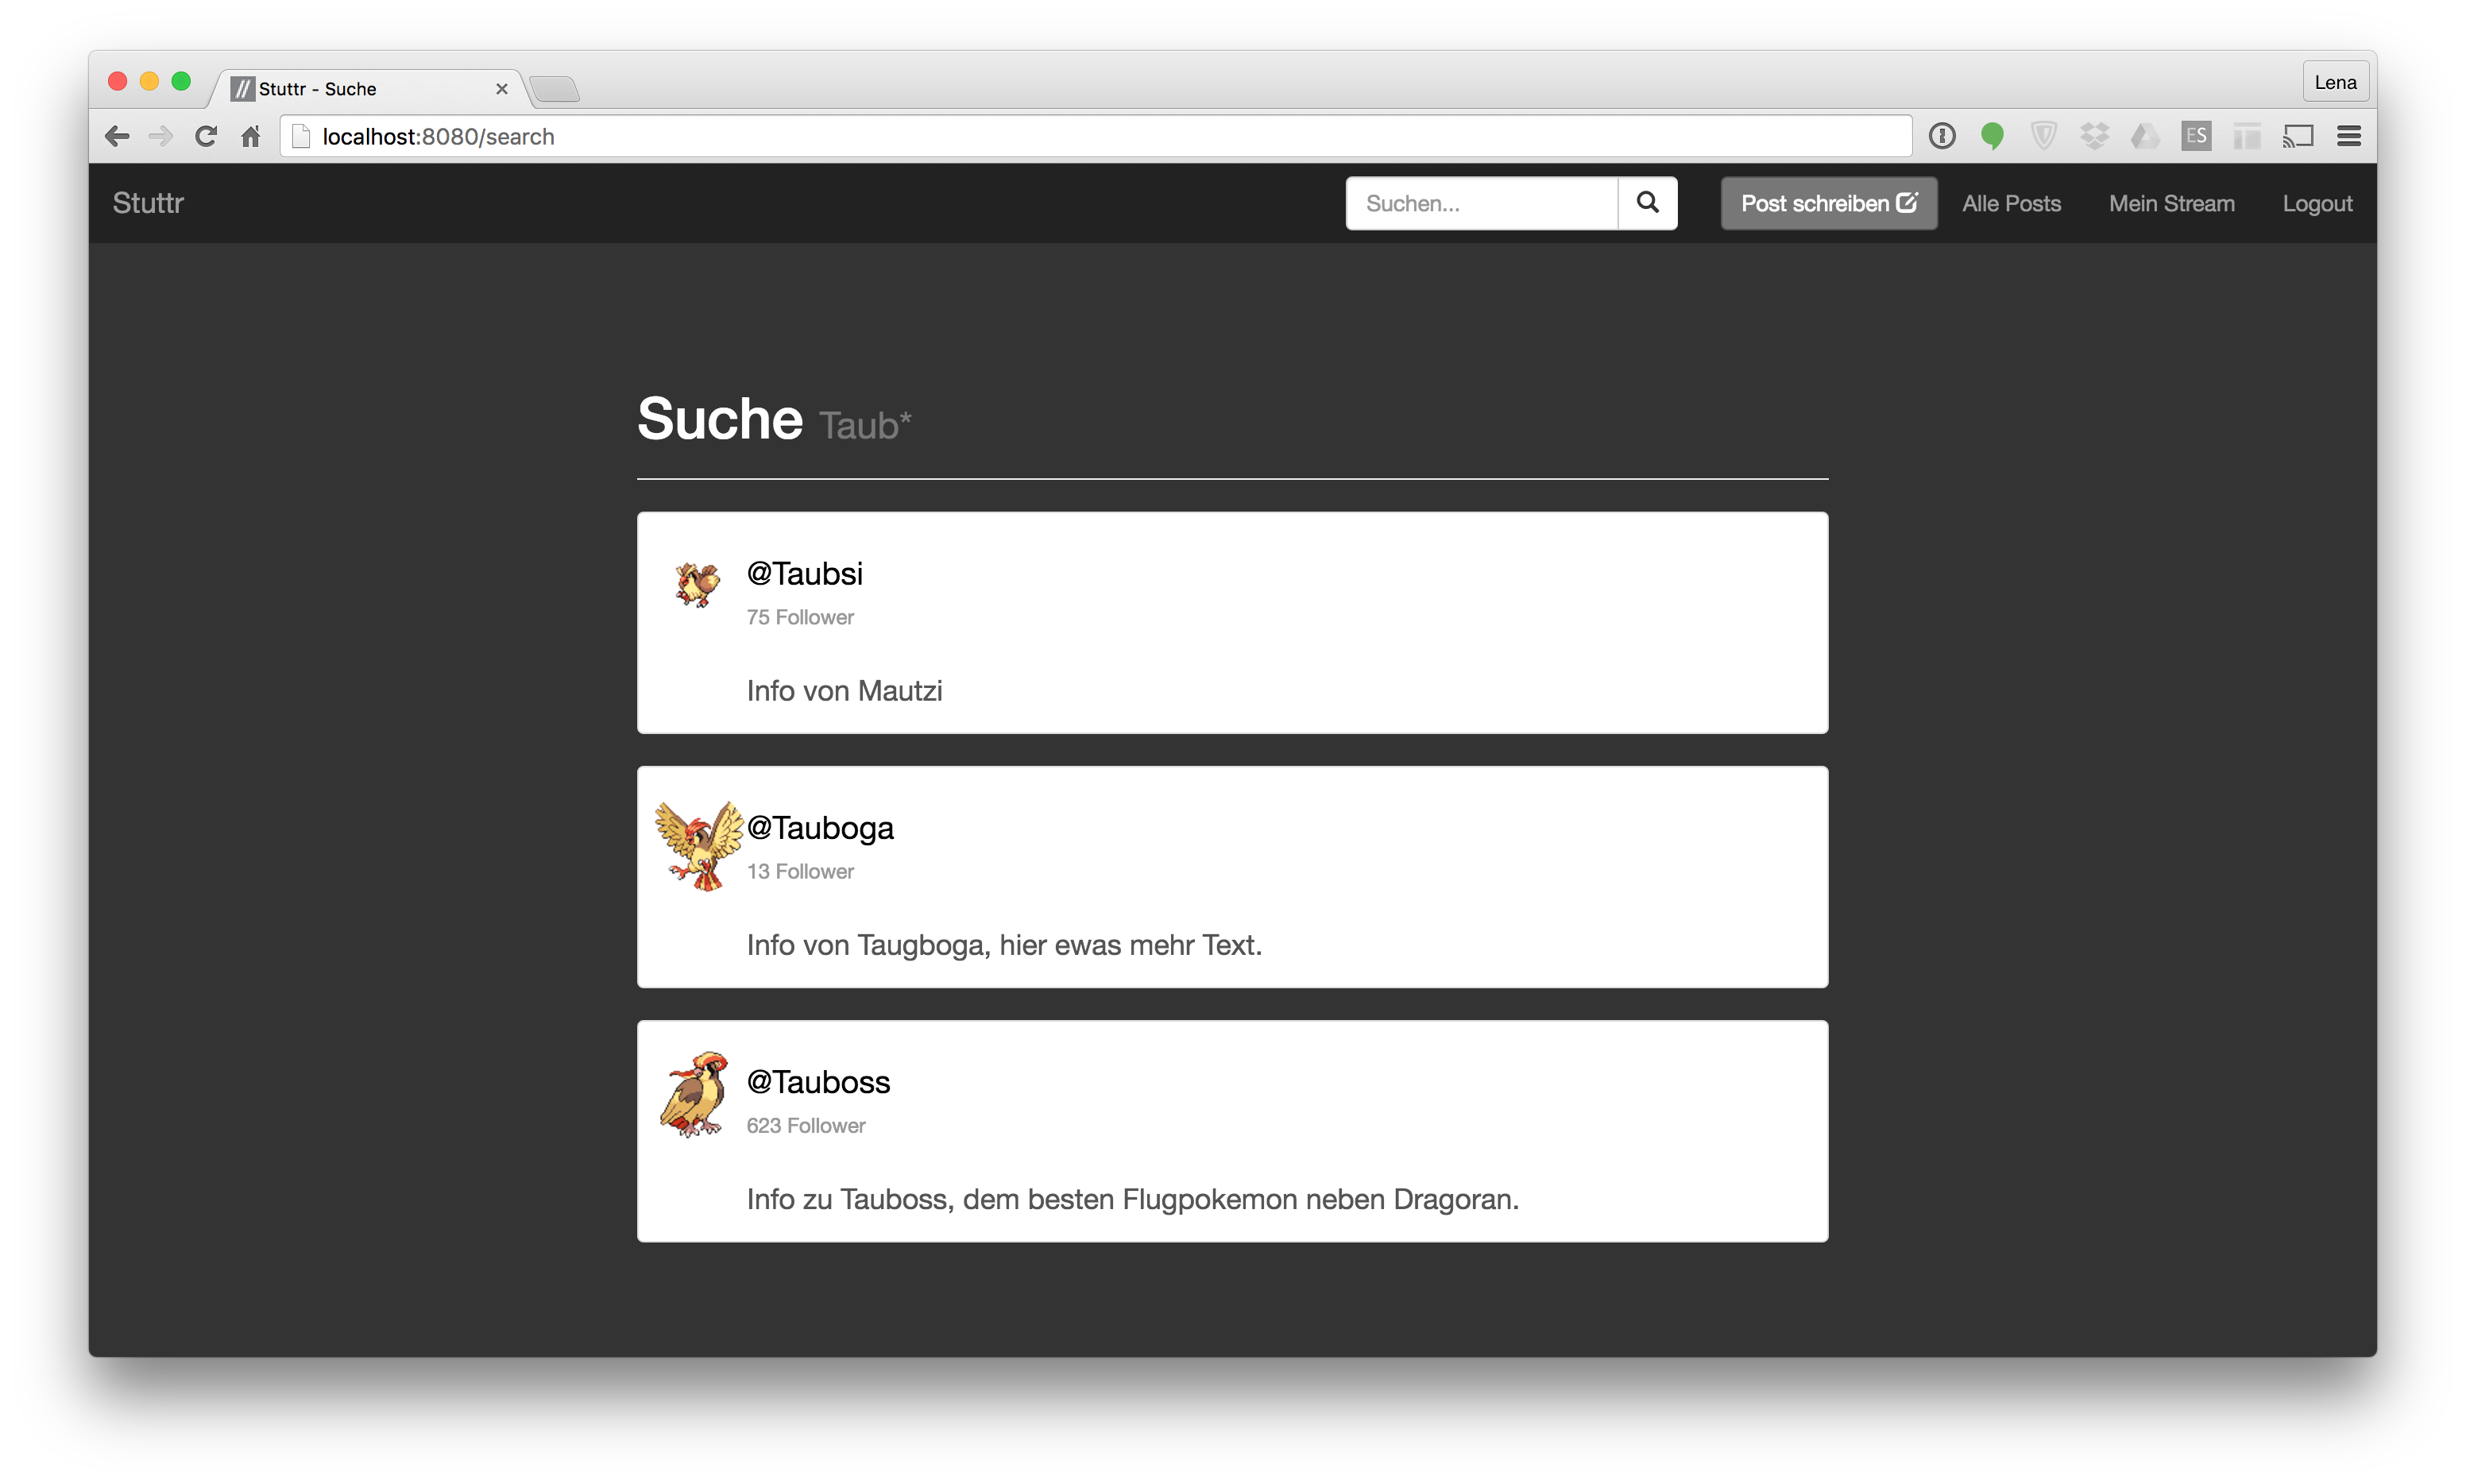
\includegraphics[width=0.8\linewidth]{search.jpg}
    \end{center}

    Die Suche wird über das Formular im Header-Bereich angesteuert. Hier kann der User einen anderen Usernamen eingeben und erhält die präsentierte Liste an anderen Usern. Um die Relevanz der Ergebnisse besser zu präsentieren, wird hier auch die Information, die ein User über sich hinterlegt hat, dargestellt, sowie die Anzahl an Followern.

    \begin{center}
      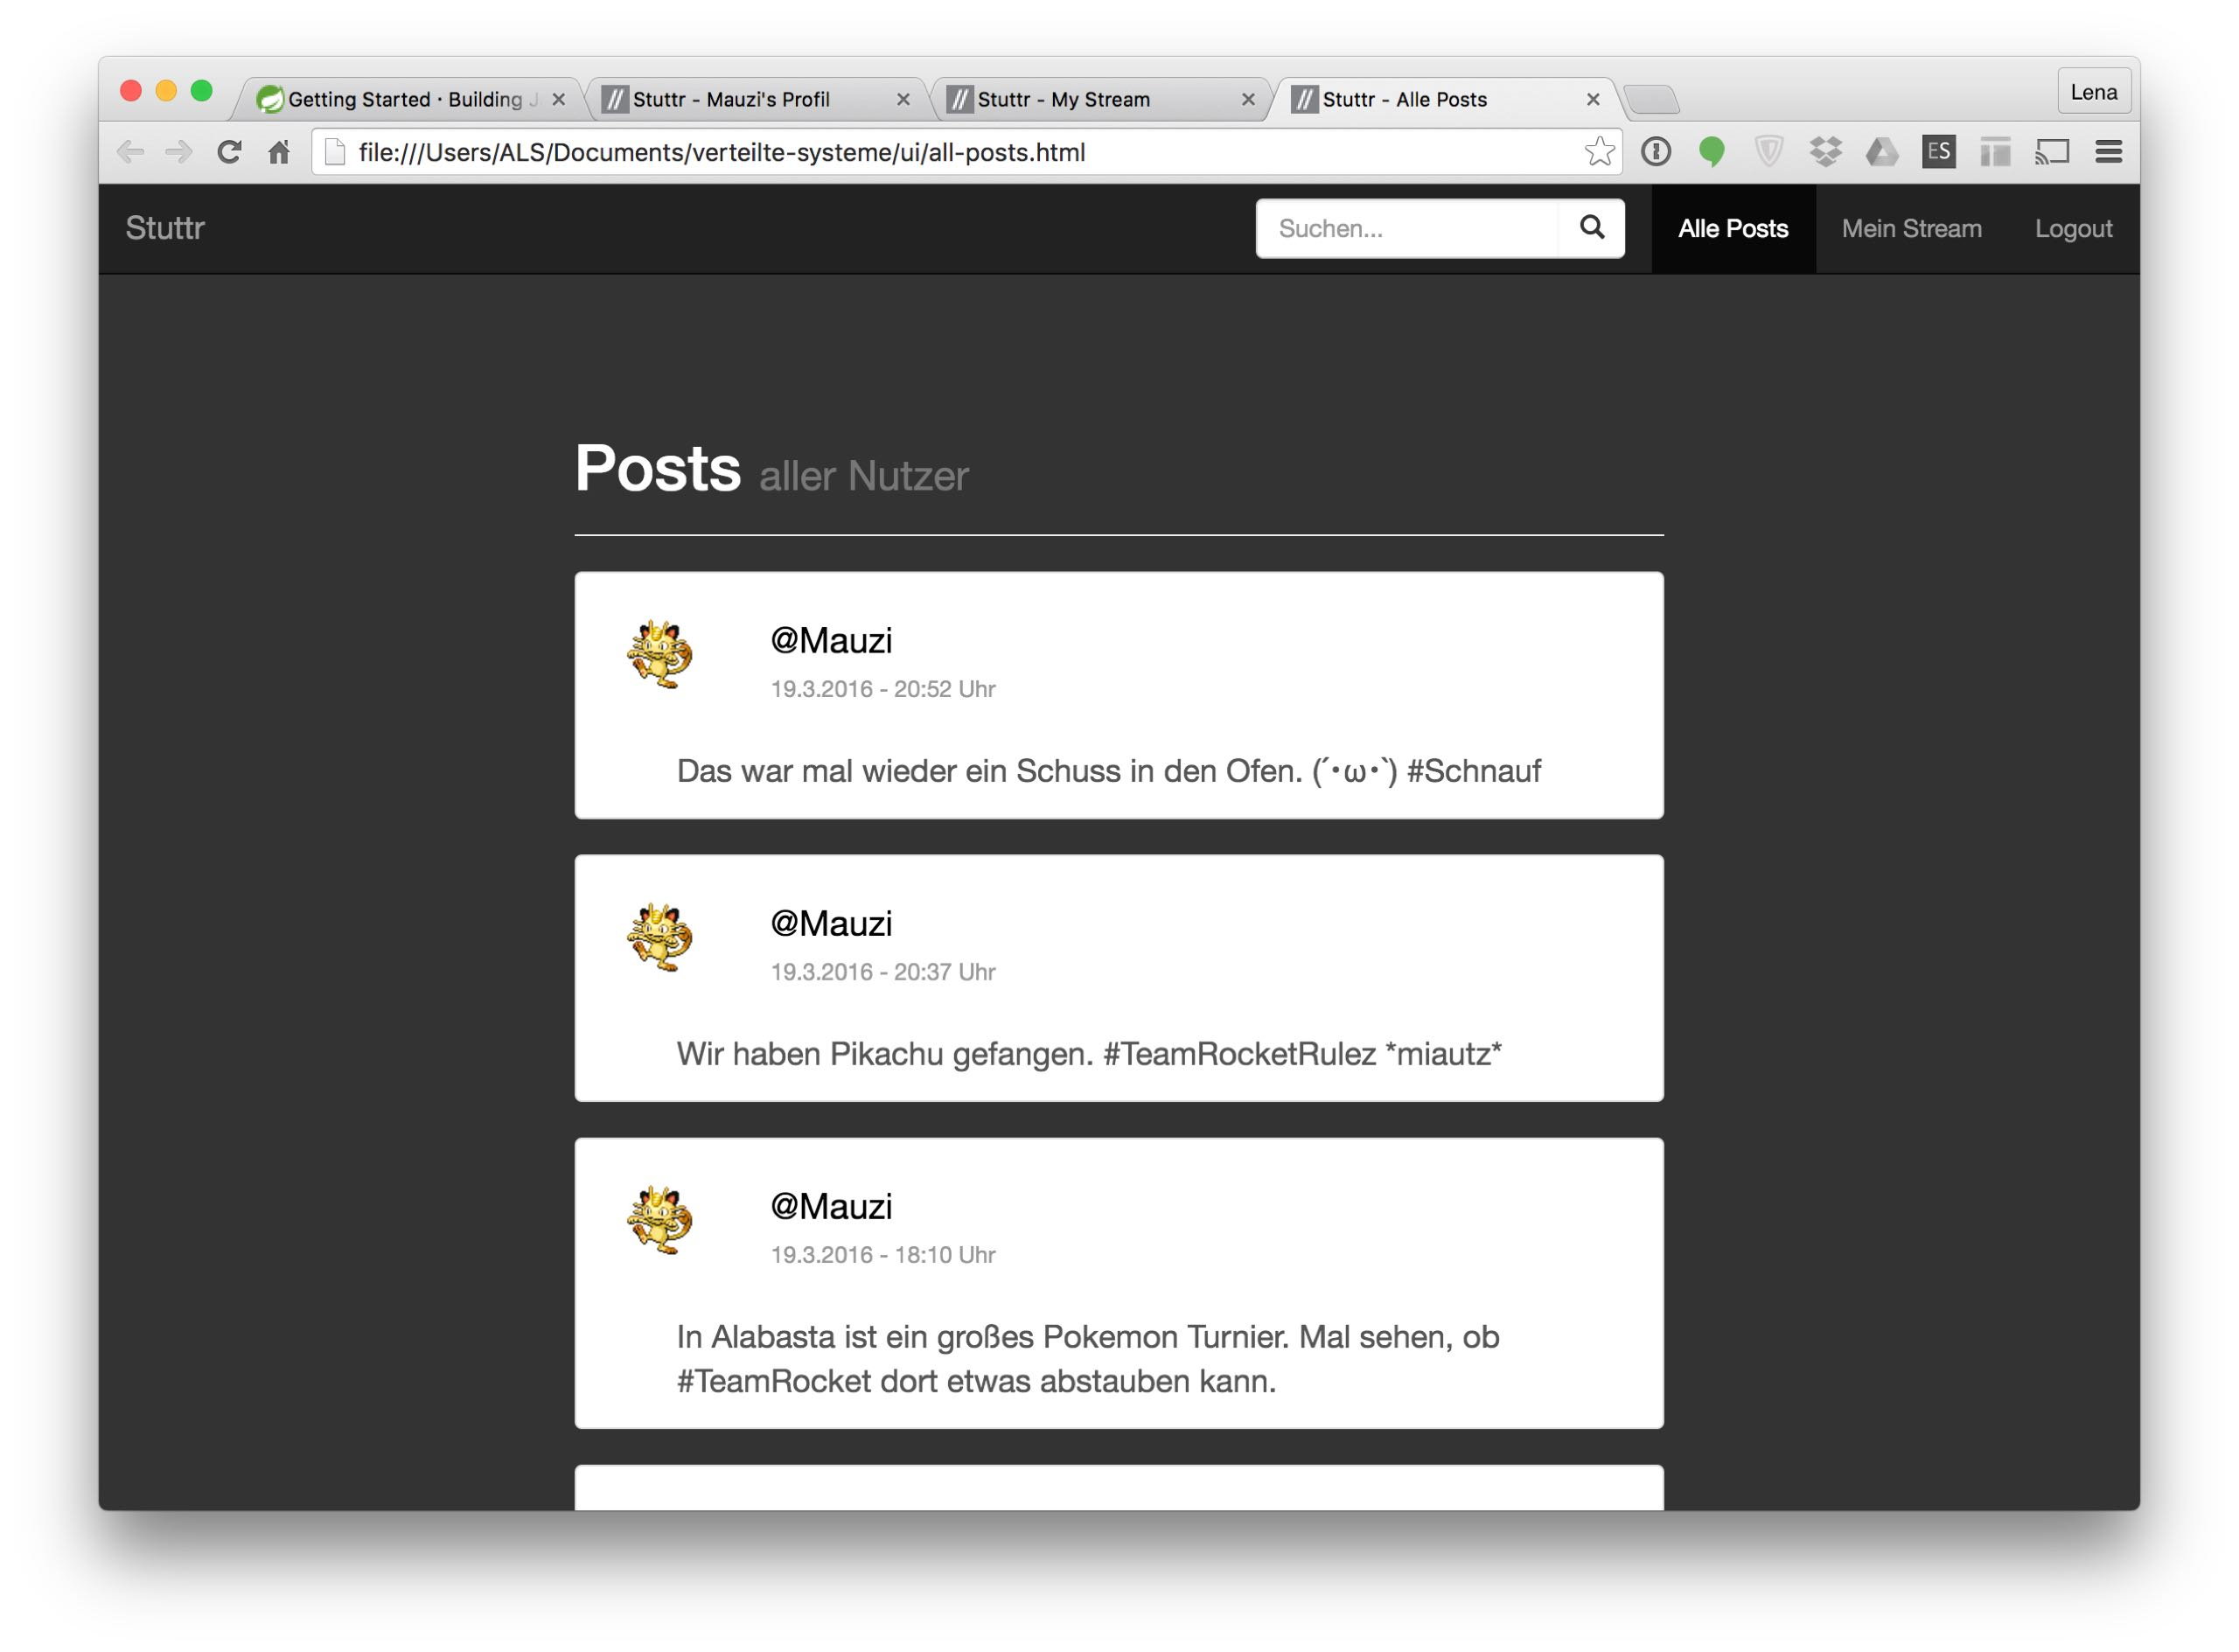
\includegraphics[width=0.8\linewidth]{all-posts.jpg}
    \end{center}

    Um sich die Posts aller User anzeigen zu lassen, kann man im Header-Menü den Punkt „Alle Posts“ anwählen und man erhält eine Ansicht aller Posts – chronologisch sortiert.

\newpage
    \begin{center}
      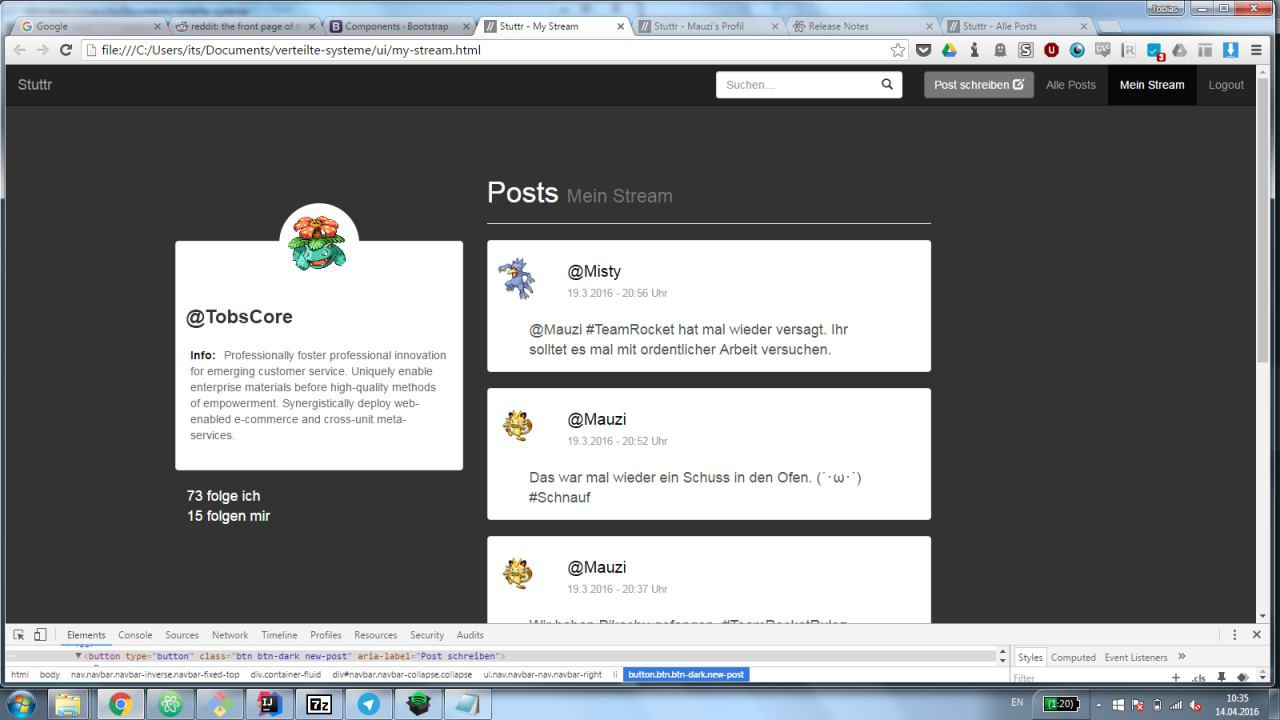
\includegraphics[width=0.8\linewidth]{my-stream.jpg}
    \end{center}

    Der Stream umfasst alle Posts von Usern, denen gefolgt wird, sowie der eigenen Posts. Hier werden auch die eigenen Informationen dargestellt und und die Liste der Posts ist auch hier wieder chronologisch sortiert.

    \begin{center}
      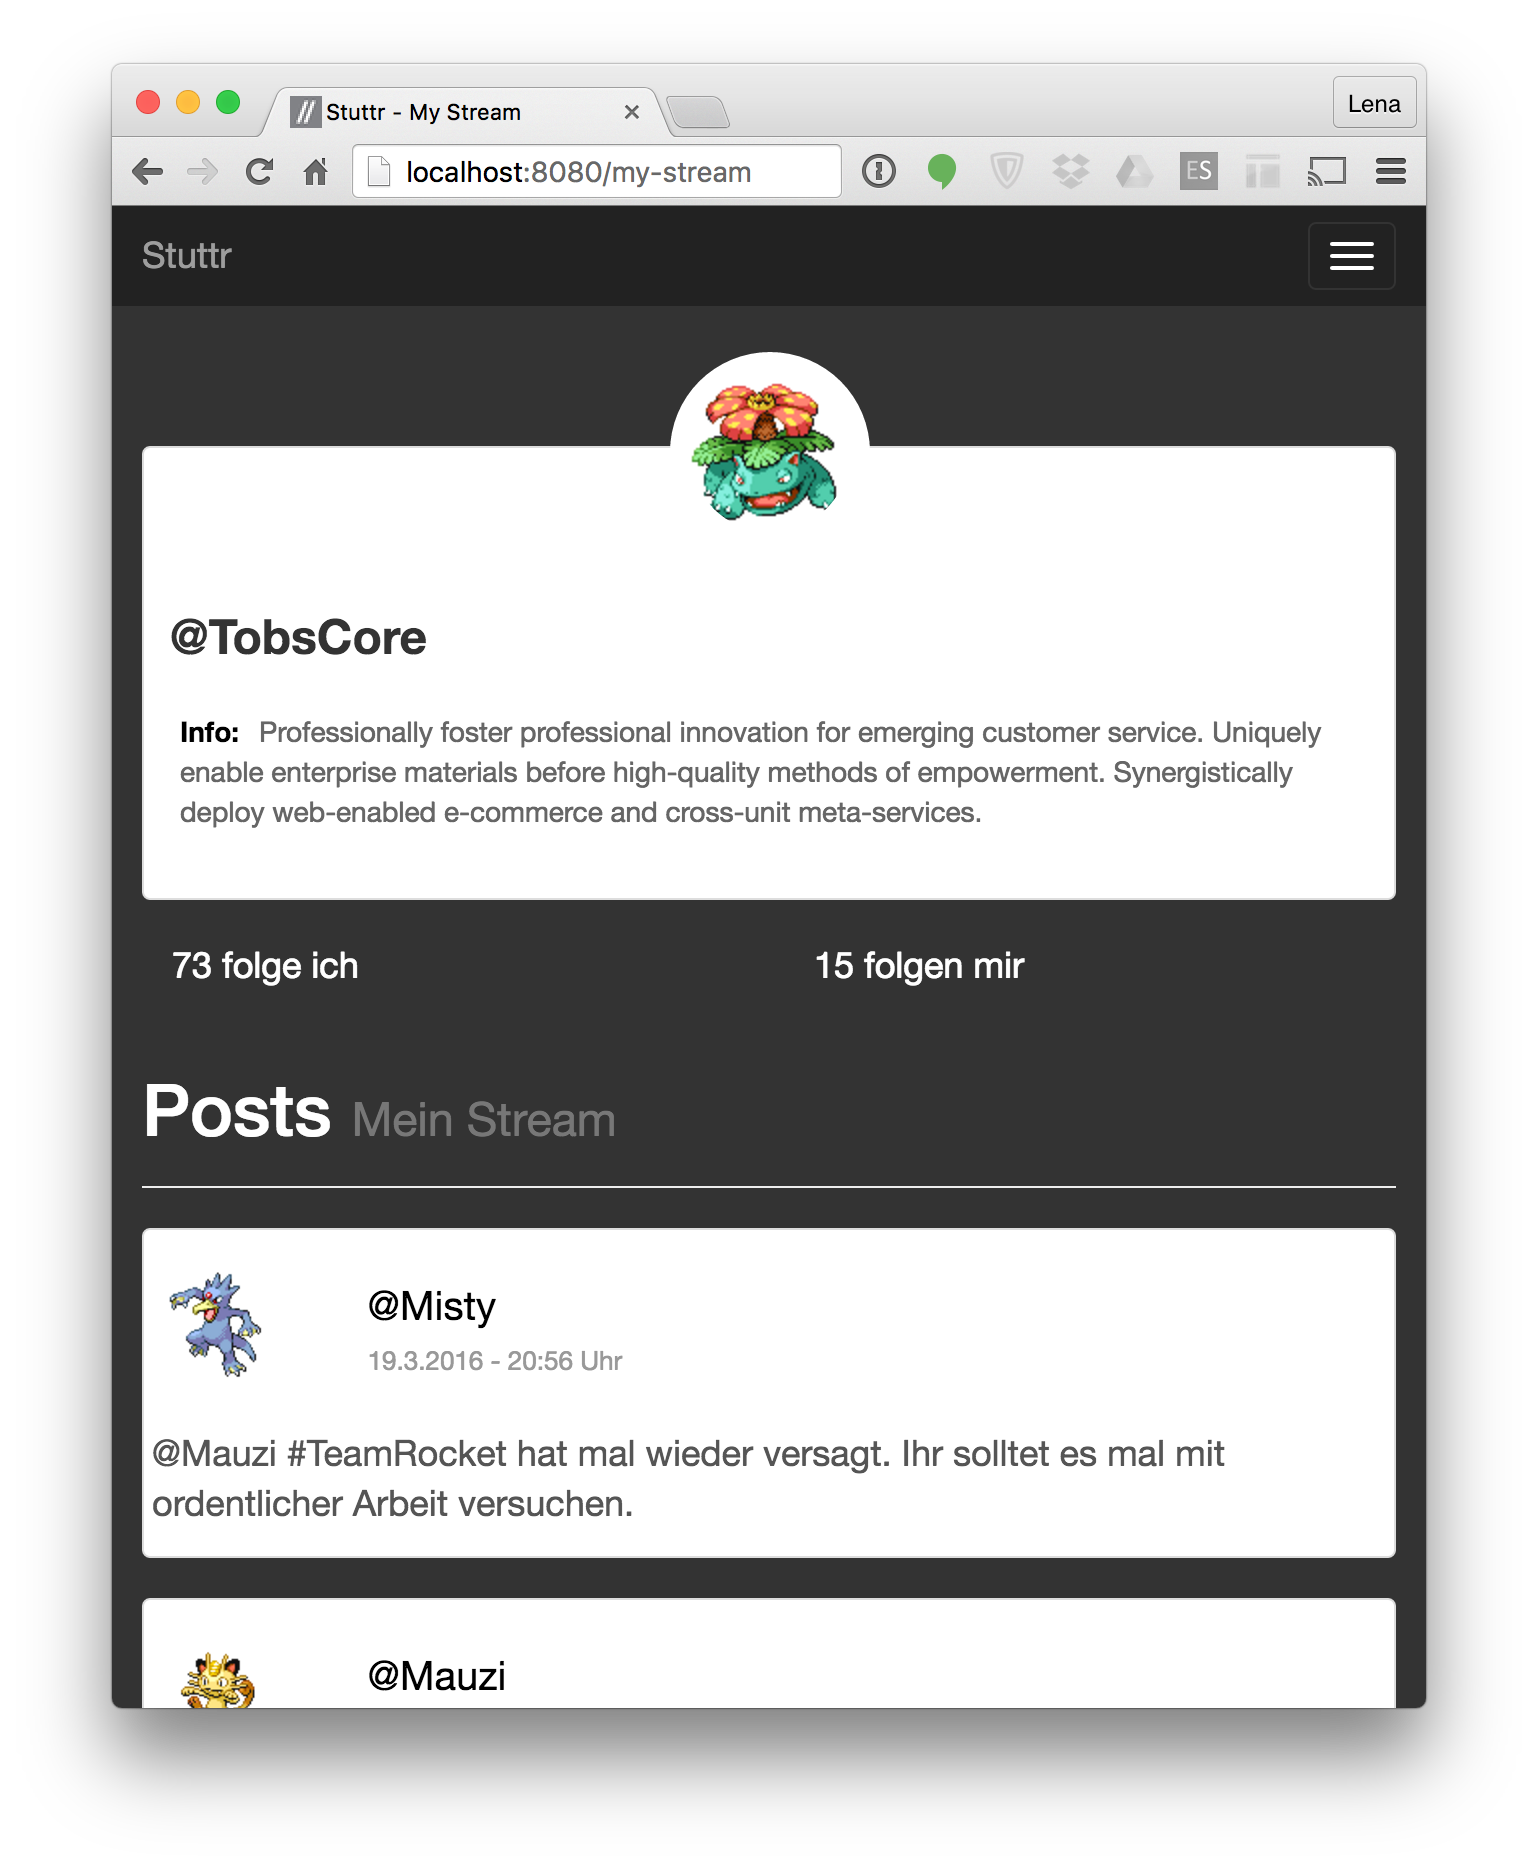
\includegraphics[width=0.75\linewidth]{my-streamResponsive.jpg}
    \end{center}

    Das Interface ist responsive. Das heißt, es passt sich an das Gerät, auf dem es benutzt wird, an. Hier haben wir exemplarisch den Stream genommen um zu zeigen, dass die Inhalte skaliert dargestellt werden. Die Design-Elemente ähneln sich zwar, sind jedoch auf die einzelnen Geräte optimiert.

\newpage
  \section{Entwurf des Datenmodells auf Basis von Redis}
  \begin{center}
    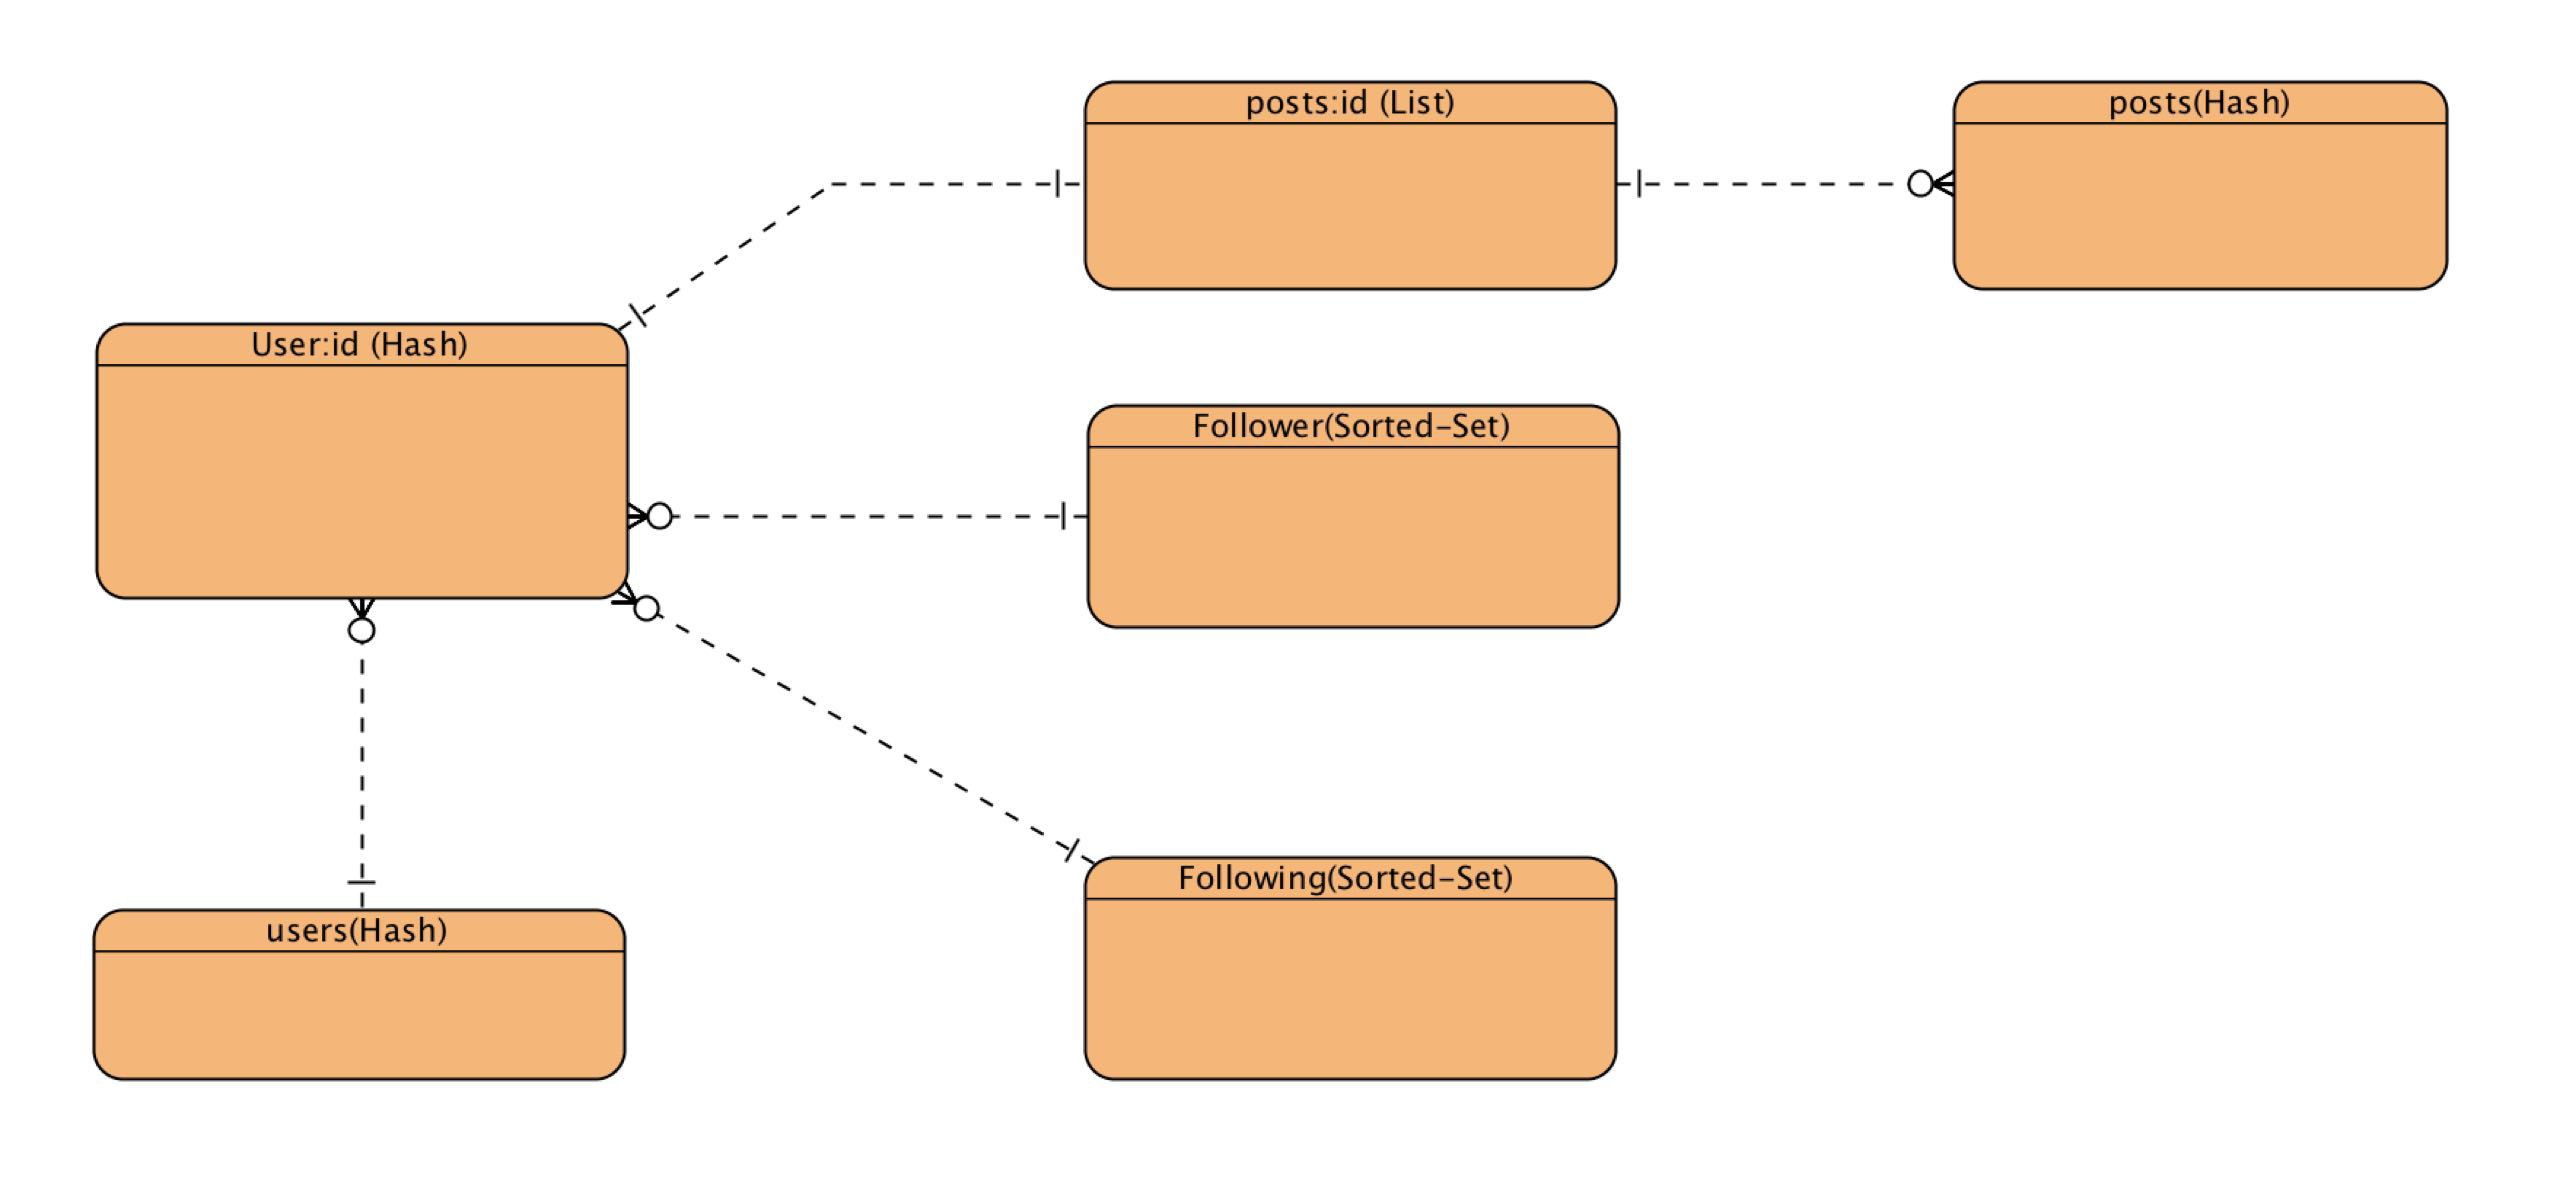
\includegraphics[width=1.0\linewidth]{redisDatenstruktur.jpg}
  \end{center}

  Die Userdaten werden in Hashs mit einzigartigen IDs im Namen verwaltet: \\
  \texttt{HMSET user: UserID (Name name, Passwort passwort)}

  Zusätzlich wird die UserID in einem Hash mit dem Usernamen als key gespeichert, sodass ein User auch über seinen Namen gefunden werden kann: \\
  \texttt{HSet users (name, id)}

  Für jeden User werden außerdem noch zwei einzigartige Sorted-Sets erstellt, um die Following-Funktion umzusetzen: \\
  \texttt{following: UserID (4123 time, 1234 time,4123 time…)} \\ ist ein Sorted-Set, das alle UserIDs und die Followingzeit der Nutzer enthält, denen der entsprechende User folgt.

  \texttt{followers: UserID(6152 time, 1342 time, 4122 time…)} \\ ist ein Sorted-Set, das alle UserIDs und die Followerzeit der Nutzer enthält, die dem entsprechenden User folgen.
  Für die Verwaltung der Kurznachrichten werden zwei weitere Datenstrukturen benötigt: \\
  \texttt{posts: UserID (56232,56233…)} \\ ist eine Liste von einzigartigen PostIDs, welche die Timeline eines Nutzers repräsentiert.
  Die Inhalte der Posts können wieder als Hash gespeichert werden, mit der einzigartigen PostID als Key und dem Inhalt als Value. \\Beispiel: \\
  \texttt{HSet posts (1, Heute war ein cooler Tag)}

\newpage
  \subsubsection{Zusammenfassung:}
  (Hash) user: UserID (Name name, Passwort passwort) \\
  (Hash) users (Name, id) \\
  (Sorted-Set) following: UserID (id, time) \\
  (Sorted-Set) followers: UserID (id, time) \\
  (List) posts: UserID (id) \\
  (Hash) posts (id, text)

\chapter{Seitenbasierte Implementierung}
\section{Überblick über die Implementierung}

\chapter{Asynchrone Erweiterungen}
\section{Überblick der Implementierung}
\subsection{Push-Funktionalität zwischen Webserver und --client}
\paragraph{Implementierung mithilfe von STOMP--over--WebSocket}
Zur Realisierung der Websocket Funktionalitäten haben wir die \texttt{Sock.js} und \texttt{Stomp.js} JavaScript Libraries in unser Projekt eingebunden. Zusätzlich mussten zusätzlich noch Dependencies in Maven anpassen, sodass die entsprechenden Klassen benutzt werden können.
\begin{verbatim}
<dependency>
    <groupId>org.springframework.boot</groupId>k
    <artifactId>spring-boot-starter-websocket</artifactId>
</dependency>
<dependency>
    <groupId>org.springframework</groupId>
    <artifactId>spring-messaging</artifactId>
</dependency>
\end{verbatim}

Auf jeder Seite, die Benachrichtigungen über neue Posts anzeigen soll, wurde dann über Javascript eine Socket Verbindung aufgebaut (mittels der \texttt{connect()} Methode aus dem Beispiel) und somit wurde dann der \texttt{Subscribe}--Mechanismus implementiert.\\
Der \texttt{Publish}--Mechanismus wurde in der HTML Seite, die zum Posten von neuen Nachrichten erstellt wurde, implementiert. Hier wird ein \texttt{JSON-Objekt} vor dem Abschicken an den Server per \texttt{AJAX} geschickt. Dieser Request wird von einem speziellen Controller verarbeitet und hierüber werden dann die abonnierenden Clients informiert.

Die Darstellung erfolgt über eine \texttt{Notification}, die anzeigt, wie viele neue Posts seit dem Aktualisieren eingagengen sind. Hierbei wird bei jeder ankommenden Nachricht geguckt, wie viele Nachrichten bisher eingangen ist und die Anzahl wird erhöht.

Beim Logout wird die Websocket-Verbindung getrennt und somit können keine weiteren Nachrichten empfangen werden.

%TODO: Lena, bitte hier einen Screenshot der Notification einfügen.
\subsection{Austausch von Updatenachrichten zwischen
Serverinstanzen}
\paragraph{Austausch über Redis Publish-Subscribe-Messaging}
Der Redis Pub-Sub Mechanismus implementiert ein Messaging-System, bei dem Publisher Nachrichten
über einen so genannten Channel senden können. Ein Redis Client kann eine beliebige Anzahl solcher Channels
abonnieren, um dort veröffentlichte Messages automatisch zu empfangen. Will ein Client die Nachrichten eines Channels
nicht mehr empfangen, so kann er diesen deabonnieren (Unsubscribe).
Für die Konfiguration unserer Anwendung, um diesen Mechanismus umzusetzen, werden in Spring, zusätzlich zu den Beans RedisTemplate und Connectionfactory,
die Beans ChannelTopic, MessageListener und RedisPublisher benötigt. Über die Annotation @Schedule kann festgelegt werden, in welchem
Zeitabstand neue Messages vom Publisher veröffentlicht werden.


\listoffigures

\end{document}
